\chapter{Випромінювання плаского диску}
\label{ch:pdisk}

%%%%%%%%%%%%%%%%%%%%%%%%%%%%%%%%%%%%%%%%%%%%%%%%%%%%%%%%%%%%%%%%%%%%%%%%%%%%%%%
\section{Постановка задачі}
%
\begin{equation}
\vect{j_0} \left( r, t \right) = \vect{J} = \vect{x_0} A_0 H(t) \delta(z) 
\left(  H(\rho) - H(\rho - R) \right)
\end{equation}
%
\begin{figure}[htbp] \begin{center}
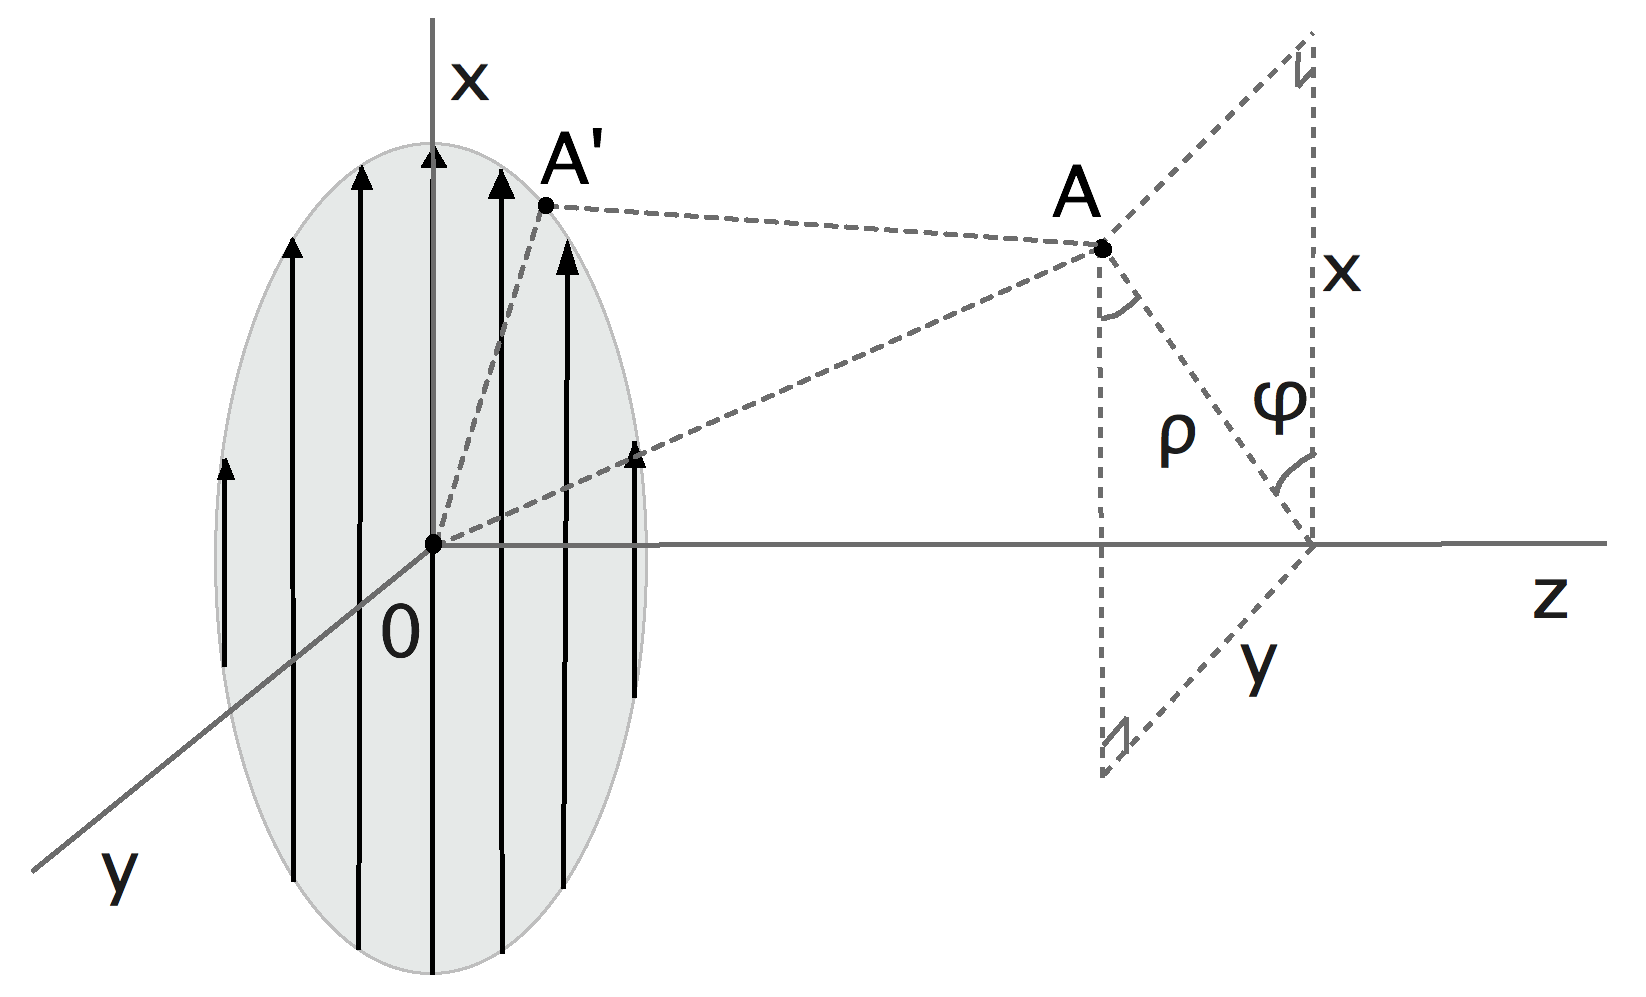
\includegraphics[scale=0.55]{PlaneDisk}
\caption{Геометрія випромінювача} \label{fig:pdisk}
\end{center} \end{figure}
%
\textcolor{lightgray} { \begin{equation*} \begin{aligned}
\begin{cases}
\vect{\rho_0} = \vect{x_0} \cos \varphi + \vect{y_0} \sin \varphi \\
\vect{\varphi_0} = - \vect{x_0} \sin \varphi + \vect{y_0} \cos \varphi
\end{cases} \Rightarrow \mathbf{A} = \left( \begin{array}{cc}
\cos \varphi & \sin \varphi \\
- \sin \varphi & \cos \varphi
\end{array} \right)
\end{aligned} \end{equation*} }
%
\textcolor{lightgray} { \begin{equation*} \begin{aligned}
\vect{j_0} \left( \vect{\rho_0}, \vect{\varphi_0} \right) = 
\mathbf{A} \vect{j_0} \left( \vect{x_0}, \vect{y_0} \right) = \\
= H(t) \delta(z) (  H(\rho) - H(\rho - R) ) 
( \vect{\rho_0} \cos \varphi - \vect{\varphi_0} \sin \varphi )
\end{aligned} \end{equation*} }
%
\begin{equation}
j_m \left( r, t; \nu \right) = \frac{\sqrt{\mu_0}}{2\pi} 
\int \limits_{0}^{2\pi} d \varphi \int \limits_{0}^{\infty} \rho d \rho 
\vect{j_0} \crossprod{ \nabla_\perp \Psi_m^* }{ \vect{z_0} }
\end{equation}
%
\textcolor{lightgray} { \begin{equation*} \begin{aligned}
\crossprod{ \nabla_\perp \Psi_m^* }{ \vect{z_0} } = 
- \sqrt{\nu} e^{-im\varphi} \left( 
\vect{\varphi_0} \frac{J_{m-1} (\nu \rho) - J_{m+1} (\nu \rho)}{2} + 
\right. \\ + \left. i m \vect{\rho_0} \frac{J_m (\nu \rho)}
{\rho \nu} \right) = - \sqrt{\nu} e^{-im\varphi} \left( 
\vect{\varphi_0} \frac{J_{m-1} (\nu \rho) - J_{m+1} (\nu \rho)}{2} + 
\right. \\ + \left. i \vect{\rho_0} \frac{J_{m-1} (\nu \rho) + 
J_{m+1} (\nu \rho)}{2} \right)
\end{aligned} \end{equation*} }
%
\textcolor{lightgray} { \begin{equation*} \begin{aligned}
\vect{j_0} \crossprod{ \nabla_\perp \Psi_m^* }{ \vect{z_0} } = 
- \sqrt{\nu} ( \cos m \varphi - i \sin m \varphi ) 
H(t) \delta(z) ( H(\rho) - H(\rho - R) ) \cdot \\ \cdot \left( 
i \frac{J_{m-1} (\nu \rho) + J_{m+1} (\nu \rho)}{2} \cos \varphi
- \frac{J_{m-1} (\nu \rho) - J_{m+1} (\nu \rho)}{2} \sin \varphi
\right)
\end{aligned} \end{equation*} }
%
\textcolor{red}{ Среда распространения и начальные условия }
%
\textcolor{lightgray} { \begin{equation*} \begin{aligned}
j_m = \frac{\sqrt{\mu_0}}{2\pi} \sqrt{\nu} \delta(z) H(t) \cdot \\
\cdot \Big( \int \limits_{0}^{2\pi} d \varphi \sin \varphi 
( \cos m \varphi - i \sin m \varphi) \int \limits_{0}^{R} 
\frac{J_{m-1} (\nu \rho) - J_{m+1} (\nu \rho)}{2} \rho d \rho - \\
- i \int \limits_{0}^{2\pi} d \varphi \cos \varphi 
( \cos m \varphi - i \sin m \varphi) \int \limits_{0}^{R} 
\frac{J_{m-1} (\nu \rho) + J_{m+1} (\nu \rho)}{2} \rho d \rho \Big)
\end{aligned} \end{equation*} }
%
\textcolor{red} { \begin{equation*} \begin{aligned}
\int \limits_{0}^{2\pi} d \varphi \sin \varphi 
( \cos m \varphi - i \sin m \varphi) = i\pi ( \delta_{m,-1} - \delta_{m,1} )
\end{aligned} \end{equation*} }
%
\textcolor{red} { \begin{equation*} \begin{aligned}
\int \limits_{0}^{2\pi} d \varphi \cos \varphi 
( \cos m \varphi - i \sin m \varphi) = \pi ( \delta_{m,-1} + \delta_{m,1} )
\end{aligned} \end{equation*} }
%
\textcolor{lightgray} { \begin{equation*} \begin{aligned}
j_m = \frac{\sqrt{\mu_0}}{2\pi} \sqrt{\nu} \delta(z) H(t) 
i\pi ( \delta_{m,-1} - \delta_{m,1} ) \int \limits_{0}^{R} 
\frac{J_{m-1} (\nu \rho) - J_{m+1} (\nu \rho)}{2} \rho d \rho - \\
- \frac{\sqrt{\mu_0}}{2\pi} \sqrt{\nu} \delta(z) H(t) 
i\pi ( \delta_{m,-1} + \delta_{m,1} ) \int \limits_{0}^{R} 
\frac{J_{m-1} (\nu \rho) + J_{m+1} (\nu \rho)}{2} \rho d \rho =
\end{aligned} \end{equation*} }
%
\textcolor{lightgray} { \begin{equation*} \begin{aligned}
= i \frac{\sqrt{\mu_0 \nu}}{4} \delta(z) H(t)
\delta_{m,-1} \int \limits_{0}^{R} \left( J_{-2} (\nu \rho) - 
J_0 (\nu \rho) \right) \rho d \rho - \\
- i \frac{\sqrt{\mu_0 \nu}}{4} \delta(z) H(t)
\delta_{m,1} \int \limits_{0}^{R} \left( J_{0} (\nu \rho) - 
J_2 (\nu \rho) \right) \rho d \rho - \\
- i \frac{\sqrt{\mu_0 \nu}}{4} \delta(z) H(t)
\delta_{m,-1} \int \limits_{0}^{R} \left( J_{-2} (\nu \rho) +  
J_0 (\nu \rho) \right) \rho d \rho - \\
- i \frac{\sqrt{\mu_0 \nu}}{4} \delta(z) H(t)
\delta_{m,1} \int \limits_{0}^{R} \left( J_{0} (\nu \rho) +
J_2 (\nu \rho) \right) \rho d \rho =
\end{aligned} \end{equation*} }
%
\textcolor{lightgray} { \begin{equation*} \begin{aligned}
= - i \frac{\sqrt{\mu_0 \nu}}{2} \delta(z) H(t) 
(\delta_{m,1} + \delta_{m,-1}) 
\int \limits_{0}^{R} \left( J_{0} (\nu \rho) + 
J_2 (\nu \rho) \right) \rho d \rho - \\
- i \frac{\sqrt{\mu_0 \nu}}{2} \delta(z) H(t) 
(\delta_{m,1} + \delta_{m,-1}) 
\int \limits_{0}^{R} \left( J_{0} (\nu \rho) -
J_2 (\nu \rho) \right) \rho d \rho = \\
= - i \frac{\sqrt{\mu_0 \nu}}{2} \delta(z) H(t) 
(\delta_{m,1} + \delta_{m,-1}) 
\int \limits_{0}^{R} J_{0} (\nu \rho) \rho d \rho
\end{aligned} \end{equation*} }
%
\textcolor{lightgray} { \begin{equation*} \begin{aligned}
\int \limits_{0}^{R} J_{0} (\nu \rho) \rho d \rho = 
\frac{1}{\nu^2} \int \limits_{0}^{R} J_{0} (\nu \rho) \nu \rho d \nu \rho =
\left. \frac{\rho J_1 (\nu \rho) }{\nu} \right|_{0}^{R} = 
\frac{R J_1 (\nu R)}{\nu}
\end{aligned} \end{equation*} }
%
\begin{equation} 
j_m (z, t; \nu) = - i R A_0 \frac{\sqrt{\mu_0}}{2} \delta(z) H(t) 
\frac{\delta_{m,1} + \delta_{m,-1}}{\sqrt{\nu}} J_1 (\nu R)
\end{equation}

%%%%%%%%%%%%%%%%%%%%%%%%%%%%%%%%%%%%%%%%%%%%%%%%%%%%%%%%%%%%%%%%%%%%%%%%%%%%%%%
\section{Лінійні коефіцієнти}

\begin{equation} \begin{aligned}
V_m^h  = - \mu \partial_{ct} (h_m)
\end{aligned} \end{equation}
%
\begin{equation} \begin{aligned}
I_m^h  = \partial_z (h_m)
\end{aligned} \end{equation}
%
\textcolor{lightgray} { \begin{equation*} \begin{aligned}
- \epsilon \partial_{ct} (V_m^h) - \partial_z I_m^h + \nu^2 h_m = 
\frac{\sqrt{\mu_0}}{2 \pi} \int_0^{2\pi} d \varphi 
\int_0^{\infty} \rho d \rho \crossprod{\vect{z_0}}{\vect{J_\perp}}
\nabla_\perp \Psi_m^* (\nu) 
\end{aligned} \end{equation*} }
%
\textcolor{red} { \begin{equation*} \begin{aligned}
\crossprod{\vect{z_0}}{\vect{J_\perp}} \nabla_\perp \Psi_m^* (\nu) =
\vect{J_\perp} \crossprod{\nabla_\perp \Psi_m^* (\nu)}{\vect{z_0}}
\end{aligned} \end{equation*} }
%
\begin{equation*} \begin{aligned}
\epsilon \partial_{ct} \left( \mu \partial_{ct} h_m \right) -
\mu^{-1} \partial_z \left( \mu  \partial_z h_m \right) + 
\nu^2 h_m = j_m (z,t,\nu) \\
\partial_{ct} =  \frac{1}{c} \partder{}{t}; 
\epsilon = \epsilon (z,t);
\mu = \mu (z,t)
\end{aligned} \end{equation*}
%
\begin{equation} \begin{aligned}
\left( \frac{\sqrt{\epsilon \mu}}{c} \right)^2 
\frac{\partial^2 h_m}{\partial t^2} - 
\frac{\partial^2 h_m}{\partial z^2} + \nu^2 h_m = j_m (z,t,\nu)
\end{aligned} \end{equation}
%
\begin{equation} \begin{aligned}
\mathit{V} = \frac{c}{\sqrt{\epsilon \mu}} 
\end{aligned} \end{equation}
%
\textcolor{red}{Функція Рімана: перевірити принцип причинності}
%
\begin{equation*}
G(t,t',z,z') = \frac{\mathit{V}}{2} H \left( \mathit{V} (t-t') - (z-z') \right)
J_0 \left( \nu \sqrt{\mathit{V}^2 (t-t')^2 - (z-z')^2} \right)
\end{equation*}
%
\begin{equation}
h_m (z, t; \nu) = \iint_S j_m (t',z') G(t,t',z,z') dt' dz'
\end{equation}
%
\textcolor{lightgray} { \begin{equation*} \begin{aligned}
h_m (z, t; \nu) = - i \mathit{V} R \frac{\sqrt{\mu_0}}{4} 
\frac{\delta_{m,1} + \delta_{m,-1}}{\sqrt{\nu}} J_1 (\nu R)
\int \limits_{0}^{\infty} \delta(z) \cdot \\ \cdot
\int \limits_{t - \frac{z}{\mathit{V}}}^{0} 
J_0 \left( \nu \sqrt{\mathit{V}^2 (t-t')^2 - (z-z')^2} \right) dt' dz' = 
i \mathit{V} R \frac{\sqrt{\mu_0}}{4} 
\frac{\delta_{m,1} + \delta_{m,-1}}{\sqrt{\nu}} J_1 (\nu R)
\cdot \\ \cdot \int \limits_{0}^{\infty} \delta(z)
\int \limits_{0}^{t - \frac{z}{\mathit{V}}} 
J_0 \left( \nu \sqrt{\mathit{V}^2 (t-t')^2 - (z-z')^2} \right) dt' dz
\end{aligned} \end{equation*} }
%
\textcolor{lightgray} { \begin{equation*} \begin{aligned}
h_m (z, t; \nu) = i \mathit{V} R \frac{\sqrt{\mu_0}}{4} 
\frac{\delta_{m,1} + \delta_{m,-1}}{\sqrt{\nu}} J_1 (\nu R)
\int \limits_{0}^{t - \frac{z}{\mathit{V}}} 
J_0 \left( \nu \sqrt{\mathit{V}^2 (t-t')^2 - z^2} \right) dt'
\end{aligned} \end{equation*} }
%
\textcolor{red}{Перевірити вірність наступної нотожності
%
\begin{equation}
h_m = \frac{i R A_0}{4} \frac{\delta_{m,1} + \delta_{m,-1}}
{\sqrt{\nu} \sqrt{\epsilon_0 \epsilon \mu}} J_1 (\nu R) 
\int \limits_{0}^{t - \frac{z}{\mathit{V}}} 
J_0 \left( \nu \sqrt{\mathit{V}^2 (t-t')^2 - z^2} \right) dt'
\end{equation} }
%
Для отримання виразу для $ V_m^h $ необовязково брати інткграл в $ h_m $ 
спробуємо спростити вираз скориставшись залкжнісю через похідну по часу.
застосуємо правило інтерування Лейбніца \textcolor{red}{[ПОСИЛАННЯ]}.
%
\begin{equation} \begin{aligned} \label{eq:leibniz_rule}
\partder{}{\theta} \int_{a(\theta)}^{b(\theta)} f(x,\theta) dx = 
\int_{a(\theta)}^{b(\theta)} \partder{f}{\theta} dx + 
f\big( b(\theta), \theta \big) \partder{b}{\theta} -
f\big( a(\theta), \theta \big) \partder{a}{\theta}
\end{aligned} \end{equation}
%
В очевидь, знадобиться похідна від функції Бесселя складного аргументу.
%
\textcolor{lightgray} { \begin{equation*} \begin{aligned}
\partder{}{t} J_0 \left( \nu \sqrt{v^2 (t-t')^2 - z} \right) = 
- \nu J_1 \left( \nu \sqrt{v^2 (t-t')^2 - z} \right) 
\partder{}{t} \sqrt{v^2 (t-t')^2 - z} = \\
-  J_1 \left( \nu \sqrt{v^2 (t-t')^2 - z} \right)
\frac{2 \nu v^2 (t-t')}{2 \sqrt{v^2 (t-t')^2 - z}} = - \nu v^2 (t-t') 
\frac{J_1 \left( \nu \sqrt{v^2 (t-t')^2 - z} \right)}
     {\sqrt{v^2 (t-t')^2 - z}}
\end{aligned} \end{equation*} }
%
\begin{equation*} \begin{aligned}
\partder{}{t} J_0 \left( \nu \sqrt{v^2 (t-t')^2 - z} \right) = - \nu v^2 (t-t') 
\frac{J_1 \left( \nu \sqrt{v^2 (t-t')^2 - z} \right)}{\sqrt{v^2 (t-t')^2 - z}}
\end{aligned} \end{equation*}
%
Відразу помічаємо, що
%
\begin{equation} \begin{aligned} \label{eq:j0_hard_perp_t}
\partder{}{t'} J_0 \left( \nu \sqrt{v^2 (t-t')^2 - z} \right) =
- \partder{}{t} J_0 \left( \nu \sqrt{v^2 (t-t')^2 - z} \right) 
\end{aligned} \end{equation}
%
Тепер застосуємо \eqref{eq:leibniz_rule} з \eqref{eq:j0_hard_perp_t} та 
отримаємо спрощення - один иінтегралів зникає
%
\textcolor{lightgray} { \begin{equation*} \begin{aligned}
\partder{}{t} \int \limits_{0}^{t - \frac{z}{v}} 
J_0 \left( \nu \sqrt{v^2 (t-t')^2 - z^2} \right) dt' = \\
= \int \limits_{0}^{t - \frac{z}{v}} 
\partder{}{t} J_0 \left( \nu \sqrt{v^2 (t-t')^2 - z^2} \right) dt' +
J_0 (0) - 0 \cdot \left( \nu \sqrt{v^2 (t-t')^2 - z^2} \right) = \\
= - \int \limits_{0}^{t - \frac{z}{v}} 
\partder{}{t'} J_0 \left( \nu \sqrt{v^2 (t-t')^2 - z^2} \right) dt' + 1 =
- \Big. J_0 \left( \nu \sqrt{v^2 (t-t')^2 - z^2} \right) \Big|_{0}^{t - \frac{z}{v}} + 1 = \\
- J_0 \left( \nu \sqrt{z^2 - z^2} \right) + J_0 \left( \nu \sqrt{v^2 t^2 - z^2} \right) + 1 = 
J_0 \left( \nu \sqrt{v^2 t^2 - z^2} \right)
\end{aligned} \end{equation*} }
%
\begin{equation} \begin{aligned}
\partder{}{t} \int \limits_{0}^{t - \frac{z}{v}} 
J_0 \left( \nu \sqrt{v^2 (t-t')^2 - z^2} \right) dt' =
J_0 \left( \nu \sqrt{v^2 t^2 - z^2} \right)
\end{aligned} \end{equation}
%
\textcolor{lightgray} { \begin{equation*} \begin{aligned}
V_m^h = - \frac{\mu}{c} \partder{h_m}{t} = 
\sqrt{\mu_0} \sqrt{\frac{\mu}{\epsilon}} \frac{iR A_0}{4} 
\frac{\delta_{m,1} + \delta_{m,-1}}{\sqrt{\nu}} J_1 (\nu R)
J_0 \left( \nu \sqrt{\mathit{V}^2 t^2 - z^2} \right)
\end{aligned} \end{equation*} }
%
Тепер можемо записати формулу для коефійієнту $ V_m^h $
%
\begin{equation}
V_m^h (z, t; \nu) = - \frac{iR A_0}{4} \sqrt{\frac{\mu_0 \mu}{\epsilon}} 
\frac{\delta_{m,1} + \delta_{m,-1}}{\sqrt{\nu}} J_1 (\nu R)
J_0 \left( \nu \sqrt{\mathit{V}^2 t^2 - z^2} \right)
\end{equation}
%
\textcolor{lightgray} { \begin{equation*} \begin{aligned}
\int \limits_{0}^{t - \frac{z}{\mathit{V}}} 
J_0 \left( \nu \sqrt{\mathit{V}^2 (t-t')^2 - z^2} 
\right) dt' = \left[ \begin{array}{cc} 
\nu \mathit{V} (t-t') = s & t' = t - \frac{ds}{\nu \mathit{V}} \\
dt' = -\frac{ds}{\nu \mathit{V}} & \\
s(0) = \nu \mathit{V} t & s \left( t - \frac{z}{\mathit{V}} \right) = \nu z
\end{array} \right] = \\ = - \frac{1}{\nu \mathit{V}} 
\int_{\nu \mathit{V} t}^{\nu z} ds 
J_0 (\sqrt{s^2 - \nu^2 z^2}) = \frac{1}{\nu \mathit{V}} 
\int_{\nu z}^{\nu \mathit{V} t} ds
J_0 (\sqrt{s^2 - \nu^2 z^2})
\end{aligned} \end{equation*} }
%
\textcolor{lightgray} { \begin{equation*} \begin{aligned}
\int_{\nu z}^{\nu \mathit{V} t} ds e^{-i0s} J_0 (\sqrt{s^2 - \nu^2 z^2}) = \\ 
= \frac{1}{i} (U_1[W_+,Z] + i U_2[W_+,Z] - U_1[W_-,Z] - i U_2[W_-,Z]) = \\
= \frac{1}{i} (-U_1[W_-,Z] + i U_2[W_+,Z] - U_1[W_-,Z] - i U_2[W_+,Z]) = \\
= \left[ \begin{array}{c} W_\pm = \pm i (\nu \mathit{V} t - \nu z) \\
Z = \sqrt{\nu^2 \mathit{V}^2 t^2 - \nu^2 z^2} \end{array} \right] = 
2i U_1 \left[ -i \nu (\mathit{V}t-z), \nu \sqrt{\mathit{V}^2 t^2-z^2} \right]
\end{aligned} \end{equation*} }
%
\textcolor{lightgray} { \begin{equation*} \begin{aligned}
\int \limits_{0}^{t - \frac{z}{\mathit{V}}} 
J_0 \left( \nu \sqrt{\mathit{V}^2 (t-t')^2 - z^2} 
\right) dt' = \frac{2i}{\nu \mathit{V}} U_1 
\left[ -i \nu (\mathit{V}t-z), \nu \sqrt{\mathit{V}^2t^2-z^2} \right]
\end{aligned} \end{equation*} }
%
\textcolor{lightgray} { \begin{equation*} \begin{aligned}
h_m (z, t; \nu) = \mathit{V} \sqrt{\mu_0} \frac{iR A_0}{4} 
\frac{\delta_{m,1} + \delta_{m,-1}} {\sqrt{\nu}} J_1 (\nu R) 
\frac{2i}{\nu \mathit{V}} U_1 \left[ W_-, Z \right]
\end{aligned} \end{equation*} }
%
\begin{equation}
h_m (z, t; \nu) = - \sqrt{\mu_0} \frac{R A_0}{2} 
\frac{\delta_{m,1} + \delta_{m,-1}}
{\nu^{3/2}} J_1 (\nu R) U_1 \left[ W_-, Z \right]
\end{equation}
%
\textcolor{lightgray} { \begin{equation*} \begin{aligned}
I_{m}^{h} = \partder{h_m}{z} = 
- \sqrt{\mu_0} \frac{R A_0}{2} 
\frac{\delta_{m,1} + \delta_{m,-1}}
{\nu^{3/2}} J_1 (\nu R) \partder{}{z} U_1 [ W_-, Z ]
\end{aligned} \end{equation*} }
%
\textcolor{lightgray} { \begin{equation*} \begin{aligned}
\begin{array}{lcr}
\derivat{W_-}{z} = i \nu & &
\derivat{Z}{z} = \frac{\nu}{2 \sqrt{\mathit{V}^2 t^2 - z^2}} (-2z) = 
- \frac{\nu z}{\sqrt{\mathit{V}^2 t^2 - z^2}} \\
\end{array}
\end{aligned} \end{equation*} }
%
\textcolor{lightgray} { \begin{equation*} \begin{aligned}
\left( \frac{Z}{W} \right)^2 = 
\left( - \frac{ \sqrt{\mathit{V}^2 t^2-z^2}}{i(\mathit{V} t-z)} \right)^2 =
\left( \frac{ i \sqrt{\mathit{V}^2 t^2-z^2}}{\mathit{V}t-z} \right)^2 =
- \frac{\mathit{V}^2 t^2-z^2}{(\mathit{V} t-z)^2} = 
- \frac{\mathit{V}t+z}{\mathit{V}t-z}
\end{aligned} \end{equation*} }
%
\textcolor{lightgray} { \begin{equation*} 
\partder{}{Z} U_n (W,Z) = - \frac{Z}{W} U_{n+1} (W,Z)
\end{equation*} }
%
\textcolor{lightgray} { \begin{equation*}
2 \partder{}{W} U_n (W,Z) = U_{n-1} (W,Z) + 
\left( \frac{Z}{W} \right)^2 U_{n+1} (W,Z)
\end{equation*} }
%
\textcolor{lightgray} { \begin{equation*} \begin{aligned}
\partder{}{z} U_1 \left[ -i \nu (ct-z), \nu \sqrt{c^2t^2-z^2} \right] =
\partder{}{z} U_1[W,Z] = \partder{U_1}{W} \derivat{W}{z} + 
\partder{U_1}{Z} \derivat{Z}{z} = \\
= \frac{i \nu}{2} \left( U_0 - \frac{ct+z}{ct-z} U_2 \right) -
\frac{\nu z}{\sqrt{c^2t^2 - z^2}} 
\left( - \frac{i \sqrt{c^2t^2-z^2}}{ct-z} \right) U_2 = \\
= \frac{i \nu}{2} U_0 - \frac{i \nu}{2} \frac{ct+z}{ct-z} U_2 +
\frac{i \nu z}{ct-z} U_2 = \\ = \frac{i \nu}{2} U_0 - \frac{i \nu}{2} U_2
\left( \frac{ct}{ct-z} + \frac{z}{ct-z} - \frac{2z}{ct-z} \right) = 
\frac{i \nu}{2} (U_0[W_-,Z] - U_2[W_-,Z])
\end{aligned} \end{equation*} }
%
\begin{equation}
I_{m}^{h} = - \sqrt{\mu_0} \frac{iR A_0}{4} 
\frac{\delta_{m,1} + \delta_{m,-1}}{\sqrt{\nu}} 
J_1 (\nu R) \left( U_0 [ W_-, Z ] - U_2 [ W_-, Z ] \right)
\end{equation}

%%%%%%%%%%%%%%%%%%%%%%%%%%%%%%%%%%%%%%%%%%%%%%%%%%%%%%%%%%%%%%%%%%%%%%%%%%%%%%%
\section{Лінійне поле}

\textcolor{lightgray} { \begin{equation*} \begin{aligned}
\vect{E_\perp} = \frac{1}{\sqrt{\epsilon_0}} \left( 
\sum \limits_{m=-\infty}^{\infty} \int \limits_{0}^{\infty} 
d \nu V_m^h \crossprod{ \nabla_\perp \Psi_m }{ \vect{z_0} } +
\sum \limits_{n=-\infty}^{\infty} \int \limits_{0}^{\infty}
d \chi V_n^e \nabla_\perp \Phi_n \right)
\end{aligned} \end{equation*} }
%
\textcolor{lightgray} { \begin{equation*} \begin{aligned}
\crossprod{ \nabla_\perp \Psi_m }{ \vect{z_0} } = 
- e^{im\varphi} \left( \vect{\varphi_0} \sqrt{\nu} 
\frac{J_{m-1} (\nu \rho) - J_{m+1} (\nu \rho)}{2} - 
i m \vect{\rho_0} \frac{J_m (\nu \rho)}{ \rho \sqrt{\nu}} \right)
\end{aligned} \end{equation*} }
%
\textcolor{lightgray} { \begin{equation*} \begin{aligned}
\vect{E_\perp} = \frac{1}{\sqrt{\epsilon_0}} \int_{0}^{\infty} 
V_{-1}^h \crossprod{ \nabla_\perp \Psi_{-1}  }{ \vect{z_0} } +
\frac{1}{\sqrt{\epsilon_0}} \int \limits_{0}^{\infty} 
V_{1}^h \crossprod{ \nabla_\perp \Psi_{1} }{ \vect{z_0} } = \\
= \frac{i R A_0}{4} \sqrt{\frac{\mu_0 \mu}{\epsilon_0 \epsilon}} 
e^{- i \varphi} \int_{0}^{\infty} \frac{J_1 (\nu R)}{\sqrt{\nu}} 
J_0 \left( \nu \sqrt{c^2 t^2 - z^2} \right) \cdot \\
\cdot \left( \vect{\varphi_0} \sqrt{\nu} 
\frac{J_2 (\nu \rho) - J_0 (\nu \rho)}{2} +
i \vect{\rho_0} \frac{J_1 (\nu \rho)}{ \rho \sqrt{\nu}} \right) - \\
+ \frac{i R A_0}{4} \sqrt{\frac{\mu_0 \mu}{\epsilon_0 \epsilon}}
e^{i \varphi} \int \limits_{0}^{\infty} \frac{J_1 (\nu R)}{ \sqrt{\nu}}
J_0 \left( \nu \sqrt{c^2 t^2 - z^2} \right) \cdot \\
\cdot \left( \vect{\varphi_0} \sqrt{\nu}
\frac{J_0 (\nu \rho) - J_2 (\nu \rho)}{2} - 
i \vect{\rho_0} \frac{J_1 (\nu \rho)}{ \rho \sqrt{\nu}} \right)
\end{aligned} \end{equation*} }
%
\textcolor{lightgray} { \begin{equation*} \begin{aligned}
E_\varphi = \frac{i R A_0}{8} \sqrt{\frac{\mu_0 \mu}{\epsilon_0 \epsilon}} 
e^{-i \varphi} \int \limits_{0}^{\infty} J_1 (\nu R)
J_0 \left( \nu \sqrt{c^2 t^2 - z^2} \right)
\left( J_2 (\nu \rho) - J_0 (\nu \rho) \right) + \\
+ \frac{i R A_0}{8} \sqrt{\frac{\mu_0 \mu}{\epsilon_0 \epsilon}} 
e^{i \varphi} \int \limits_{0}^{\infty} J_1 (\nu R)
J_0 \left( \nu \sqrt{c^2 t^2 - z^2} \right)
\left( J_0 (\nu \rho) - J_2 (\nu \rho) \right) = \\
= \frac{i R A_0}{4} \sqrt{\frac{\mu_0 \mu}{\epsilon_0 \epsilon}}
\frac{e^{i \varphi} - e^{-i \varphi} }{2} \int \limits_{0}^{\infty} 
J_1 (\nu R) J_0 \left( \nu \sqrt{c^2 t^2 - z^2} \right) 
\left( J_0 (\nu \rho) - J_2 (\nu \rho) \right) =
\end{aligned} \end{equation*} }
%
\textcolor{lightgray} { \begin{equation*} \begin{aligned}
= \frac{R A_0}{4} \sqrt{\frac{\mu_0 \mu}{\epsilon_0 \epsilon}} 
\frac{e^{i \varphi} - e^{-i \varphi} }{2i} \int \limits_{0}^{\infty} 
J_1 (\nu R) J_0 \left( \nu \sqrt{c^2 t^2 - z^2} \right) 
\left( J_2 (\nu \rho) - J_0 (\nu \rho) \right) = \\
= \frac{R A_0}{4} \sqrt{\frac{\mu_0 \mu}{\epsilon_0 \epsilon}} \sin \varphi 
\int \limits_{0}^{\infty} J_1 (\nu R) 
J_0 \left( \nu \sqrt{c^2 t^2 - z^2} \right) 
\left( J_2 (\nu \rho) - J_0 (\nu \rho) \right)
\end{aligned} \end{equation*} }
%
\textcolor{lightgray} { \begin{equation*} \begin{aligned}
J_2 (\nu \rho) - J_0 (\nu \rho) = \frac{2}{\nu \rho} J_1 (\nu \rho) - 
2 J_0 (\nu \rho)
\end{aligned} \end{equation*} }
%
\textcolor{lightgray} { \begin{equation*} \begin{aligned}
E_\varphi = \frac{R A_0}{2} \sqrt{\frac{\mu_0 \mu}{\epsilon_0 \epsilon}}
\sin \varphi \int \limits_{0}^{\infty} J_1 (\nu R) 
J_0 \left( \nu \sqrt{c^2 t^2 - z^2} \right) 
\left( \frac{J_1 (\nu \rho)}{\nu \rho} - J_0 (\nu \rho) \right)
\end{aligned} \end{equation*} }
%
\textcolor{lightgray} { \begin{equation*} \begin{aligned}
E_\rho = \frac{i R A_0}{4} \sqrt{\frac{\mu_0 \mu}{\epsilon_0 \epsilon}}  
e^{- i \varphi} \int \limits_{0}^{\infty} \frac{J_1 (\nu R)}{\sqrt{\nu}} 
J_0 \left( \nu \sqrt{c^2 t^2 - z^2} \right) 
\left( - i \frac{J_1 (\nu \rho)}{\rho \sqrt{\nu}} \right) + \\
+ \mu \frac{i R A_0}{4} \sqrt{\frac{\mu_0}{\epsilon_0}}  e^{i \varphi}
\int \limits_{0}^{\infty} \frac{J_1 (\nu R)}{\sqrt{\nu}}
J_0 \left( \nu \sqrt{c^2 t^2 - z^2} \right) 
\left( - i \frac{J_1 (\nu \rho)}{ \rho \sqrt{\nu}} \right) = \\
= \mu \frac{R A_0}{2} \sqrt{\frac{\mu_0 \mu}{\epsilon_0 \epsilon}} 
\frac{e^{i \varphi} + e^{-i \varphi}}{2}
\int \limits_{0}^{\infty} \frac{J_1 (\nu R)}{\sqrt{\nu}}
J_0 \left( \nu \sqrt{c^2 t^2 - z^2} \right) 
\frac{J_1 (\nu \rho)}{ \rho \sqrt{\nu}} = \\
= \mu \frac{R A_0}{2} \sqrt{\frac{\mu_0 \mu}{\epsilon_0 \epsilon}} 
\cos \varphi \int \limits_{0}^{\infty} \frac{d \rho}{\nu \rho} 
J_1 (\nu \rho) J_1 (\nu R) J_0 \left( \nu \sqrt{c^2 t^2 - z^2} \right)
\end{aligned} \end{equation*} }
%
\begin{equation} \label{eq:linear_e_cyl}
\vect{E} \left( r, t \right) = \frac{A_0}{2} 
\sqrt{\frac{\mu_0 \mu}{\epsilon_0 \epsilon}}
\Big( \vect{\rho_0} I_1 \cos \varphi - 
\vect{ \varphi_0 } \left( I_2 - I_1 \right) \sin \varphi \Big)
\end{equation}
%
\begin{equation*}
I_1 = R \int \limits_{0}^{\infty} \frac{d \nu}{\nu \rho} J_1 (\nu \rho) 
J_1 (\nu R) J_0 \left( \nu \sqrt{\frac{c^2 t^2}{\epsilon \mu} - z^2} \right)
\end{equation*}
%
\begin{equation*}
I_2 = R \int_{0}^{\infty} d \nu J_1 (\nu R) 
J_0 (\nu \rho) J_0 \left( \nu \sqrt{\frac{c^2 t^2}{\epsilon \mu} - z^2} \right)
\end{equation*}
%
\textcolor{red} { Правильній перехід до декартових векторних кординат? } 
%
\textcolor{lightgray} { \begin{equation*} \begin{aligned}
\mathbf{A} = \left( \begin{array}{cc}
\cos \varphi & \sin \varphi \\
- \sin \varphi & \cos \varphi
\end{array} \right) \begin{array}{ccc}
	& \det A = 1 		&	\\
	& A^{-1} = A^{T}	&
\end{array} 
\mathbf{A^{-1}} = \left( \begin{array}{cc}
\cos \varphi & - \sin \varphi \\
\sin \varphi & \cos \varphi
\end{array} \right) 
\end{aligned} \end{equation*} }
%
\textcolor{lightgray} { \begin{equation*} \begin{aligned}
\vect{E} = 
\mathbf{A^{-1}} \vect{E} \left( \vect{\rho_0}, \vect{\varphi_0} \right) = 
\frac{A_0}{2} \sqrt{\frac{\mu_0 \mu}{\epsilon_0 \epsilon}}
\left( \begin{array}{cc} \cos \varphi & - \sin \varphi \\
\sin \varphi & \cos \varphi \end{array} \right)
\left( \begin{array}{c} I_1 \cos \varphi \\
- (I_2 - I_1) \sin \varphi \end{array} \right) = \\
= \frac{A_0}{2} \sqrt{\frac{\mu_0 \mu}{\epsilon_0 \epsilon}}
\left( \begin{array}{c} I_1 \cos^2 \varphi + (I_2 - I_1) \sin^2 \varphi \\
I_1 \sin \varphi \cos \varphi - (I_2 - I_1) 
\sin \varphi \cos \varphi \end{array} \right)
\end{aligned} \end{equation*} }
%
\begin{equation*} \begin{aligned}
\vect{E} \left( \vect{x_0}, \vect{y_0} \right) = \frac{A_0}{2} 
\sqrt{\frac{\mu_0 \mu}{\epsilon_0 \epsilon}} \left( \begin{array}{c} 
I_1 \cos^2 \varphi + (I_2 - I_1) \sin^2 \varphi \\
I_1 \sin \varphi \cos \varphi - (I_2 - I_1) 
\sin \varphi \cos \varphi \end{array} \right)
\end{aligned} \end{equation*}
%
Для зони $ S_3 $ тільки $ E_x $ компонента електричного поля не дорівнює
нулю. Окрім того амплітуда $ E_x $ постійна для всіх подій з облсті $ S_3 $.
%
\begin{equation*} \begin{aligned}
\vect{E} = \vect{x_0} \frac{A_0}{4} 
\sqrt{\frac{\mu_0 \mu}{\epsilon_0 \epsilon}}
\end{aligned} \end{equation*}
%
\begin{figure}[h] \begin{center}
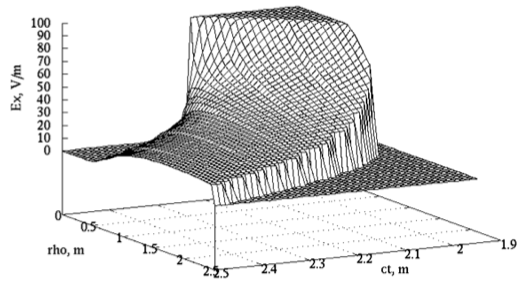
\includegraphics[scale=0.6]{MissileEffect}
\caption{Ефект електромагнітного снаряду ($ z = 2 $ м)} \label{fig:emp_rho}
\end{center} \end{figure}
%
Такий ефект носить назву електромагнітного знаряду. Хоча поле в явному
виді не залежить від точки спостереження, залежність присутня в визначенні 
зон випромінювання поля плаского диску. Користуючить ними можна вирахувати 
тривалість ефекту.
%
\begin{equation*} \begin{aligned}
\frac{c \tau}{\sqrt{\epsilon \mu}} = \sqrt{R^2+z^2} - z.
\end{aligned} \end{equation*}
%
При $ R = 1 $ можна ввести апроксимацію цієї формули, як  
%
\begin{equation*} \begin{aligned}
\frac{c \tau}{\sqrt{\epsilon \mu}} \left( z \gg 2R \right) \approx 
\begin{cases}
\frac{2R}{z} , R \geq 1 \\
\frac{R^2}{2z} , R \leq 1
\end{cases}
\end{aligned} \end{equation*}
%
\begin{figure}[h] \begin{center}
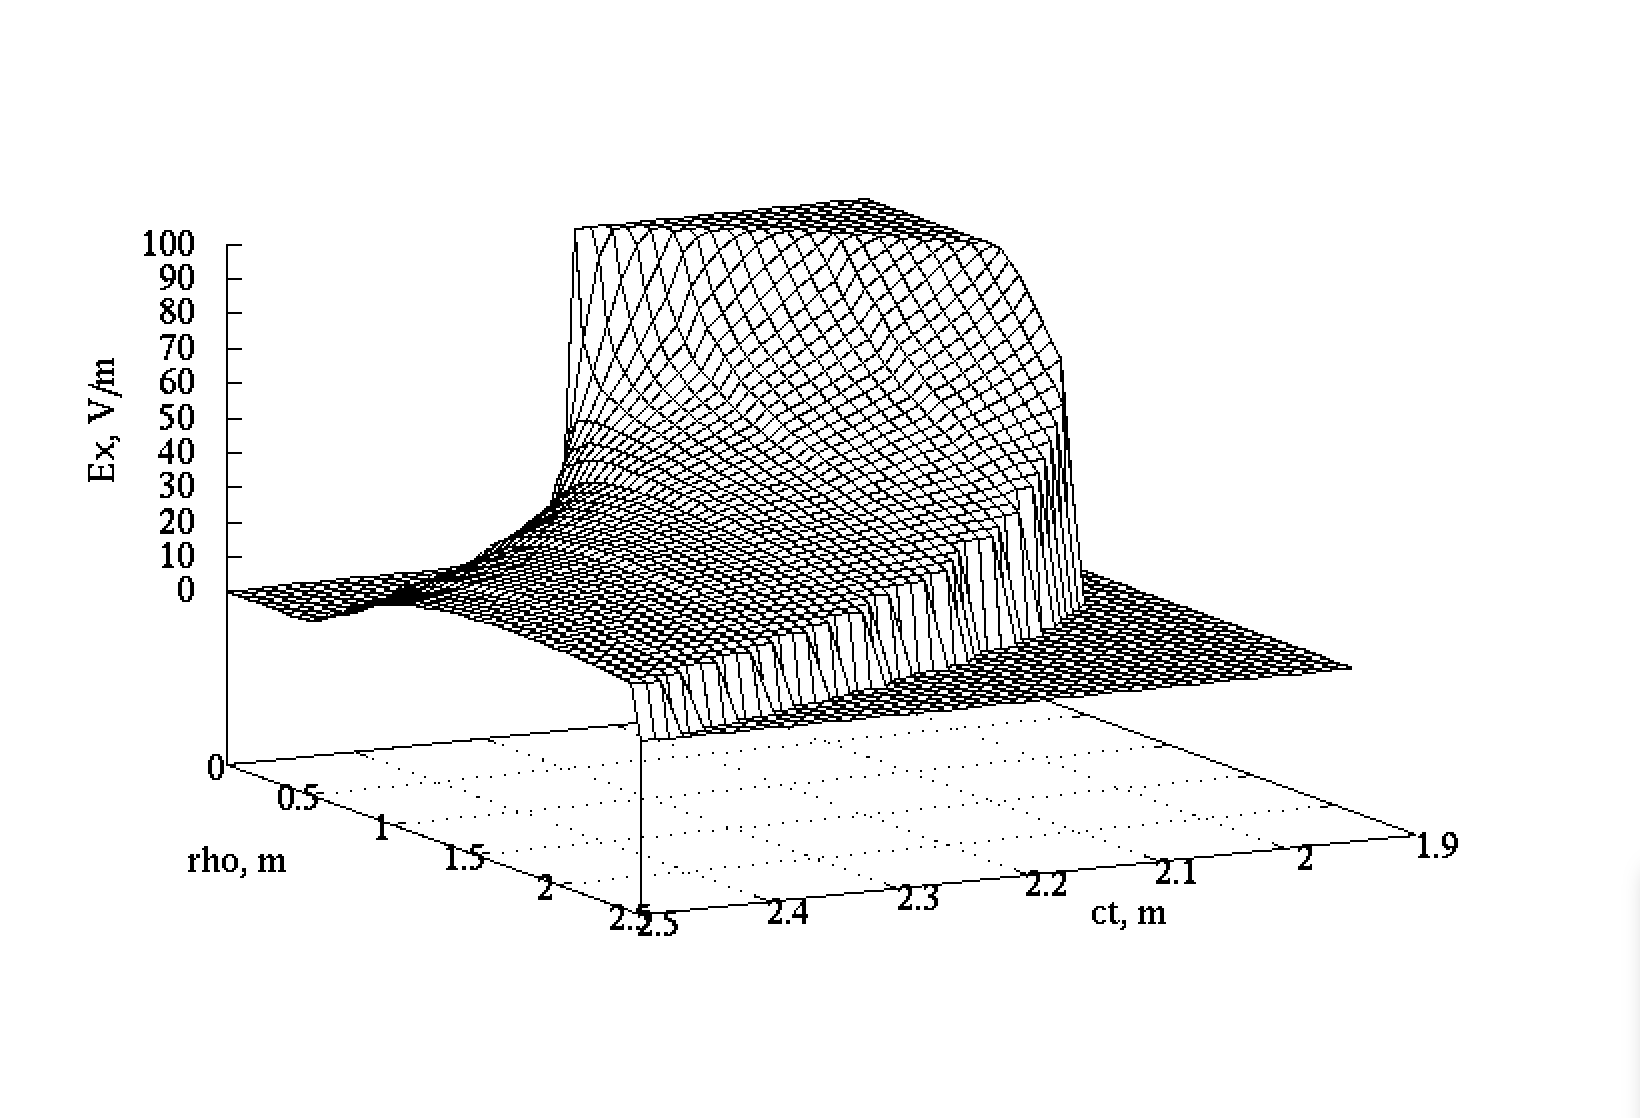
\includegraphics[scale=0.6]{TransientEffect}
\caption{Ефект електромагнітного снаряду ($ \rho = 0.2 $ м)} \label{fig:emp_z}
\end{center} \end{figure}
%
\begin{figure}[h] \begin{center}
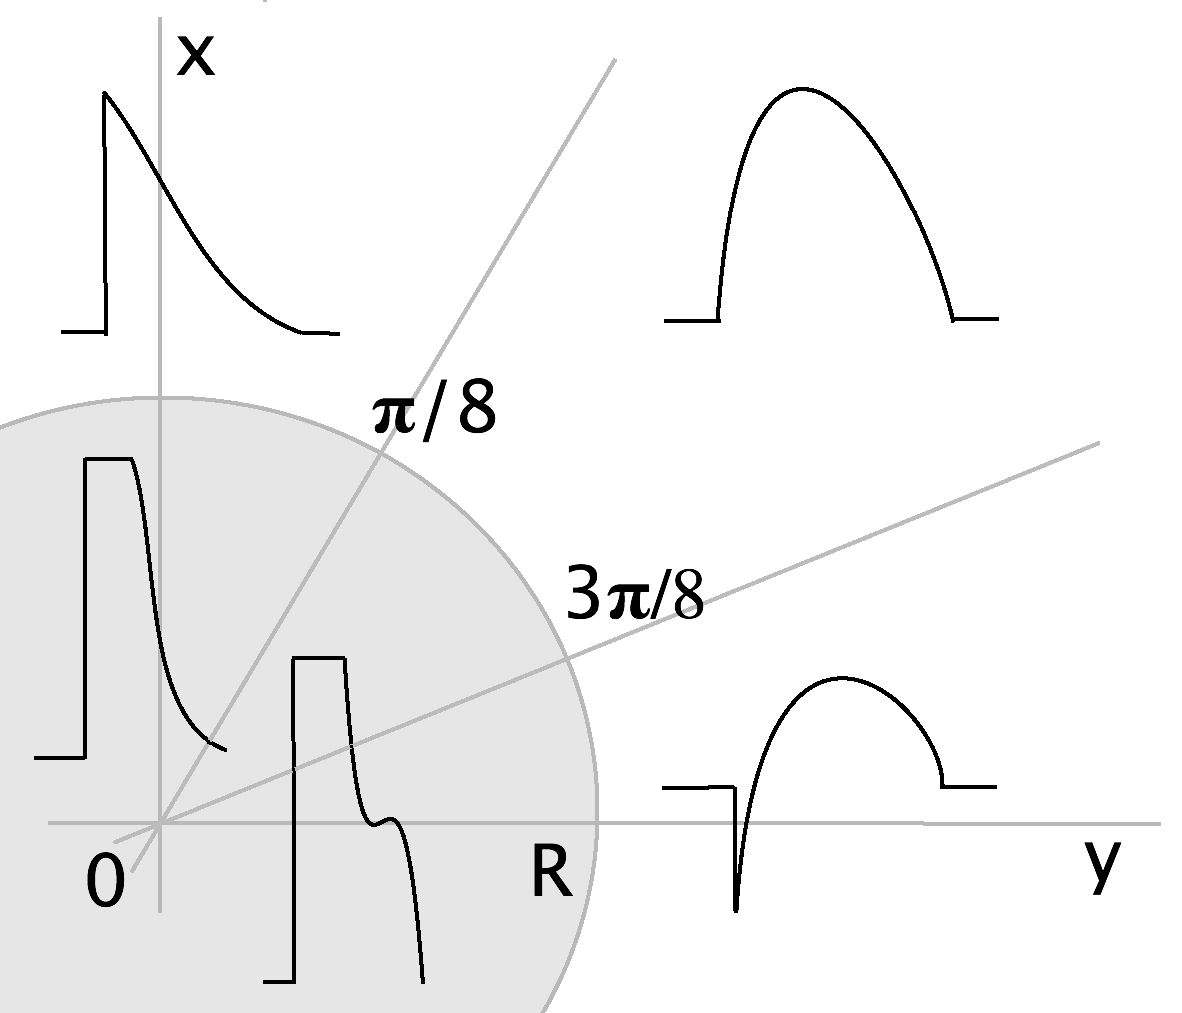
\includegraphics[scale=0.7]{LinearPulsShape}
\caption{Кутова залежнысть формы імпульсу ($ \rho = R/2 .. 2R $ м)} 
\label{fig:emp_shape}
\end{center} \end{figure}
%
\textcolor{lightgray} { \begin{equation*} \begin{aligned}
\vect{H_\perp} = \frac{1}{\sqrt{\mu_0}} \left( 
\sum \limits_{m=-\infty}^{\infty} \int \limits_{0}^{\infty} d \nu
I_m^h \nabla_\perp \Psi_m + \sum \limits_{n=-\infty}^{\infty}
\int \limits_{0}^{\infty} d \chi I_n^e 
\crossprod{\vect{z_0}}{\nabla_\perp \Phi_n} \right)
\end{aligned} \end{equation*} }
%
\textcolor{lightgray} { \begin{equation*} \begin{aligned}
\nabla_\perp \Psi_m = e^{i m \varphi} \left( \vect{\rho_0} 
\sqrt{\nu} \frac{ J_{m-1}(\nu \rho) - J_{m+1}(\nu \rho) }{2} +
i m \vect{\varphi_0} \frac{J_m(\nu \rho)}{\sqrt{\nu} \rho} \right)
\end{aligned} \end{equation*} }
%
\textcolor{lightgray} { \begin{equation*} \begin{aligned}
\vect{H_\perp} = \frac{1}{\sqrt{\mu_0}} \left( 
\int \limits_{0}^{\infty} d \nu I_{-1}^h \nabla_\perp \Psi_{-1} +
\int \limits_{0}^{\infty} d \nu I_1^h \nabla_\perp \Psi_1 \right) = \\
= - \frac{A_0}{\sqrt{\mu_0}} \int \limits_{0}^{\infty} d \nu
\sqrt{\mu_0} \frac{iR}{4} J_1 (\nu R)
\frac{ U_0 [ W_-, Z ] - U_2 [ W_-, Z ] }{\sqrt{\nu}}  
e^{- i \varphi} \cdot \\ \cdot \left( \vect{\rho_0} 
\sqrt{\nu} \frac{ J_{2}(\nu \rho) - J_{0}(\nu \rho) }{2} +
i \vect{\varphi_0} \frac{J_1(\nu \rho)}{\sqrt{\nu} \rho} \right) -
\frac{A_0}{\sqrt{\mu_0}} \int \limits_{0}^{\infty} d \nu 
\sqrt{\mu_0} \frac{iR}{4} J_1 (\nu R) \cdot \\
\cdot \frac{ U_0 [ W_-, Z ] - U_2 [ W_-, Z ] }{\sqrt{\nu}} 
e^{i \varphi} \left( \vect{\rho_0} 
\sqrt{\nu} \frac{ J_{0}(\nu \rho) - J_{2}(\nu \rho) }{2} +
i \vect{\varphi_0} \frac{J_1(\nu \rho)}{\sqrt{\nu} \rho} \right)
\end{aligned} \end{equation*} }
%
\textcolor{lightgray} { \begin{equation*} \begin{aligned}
H_\varphi = \frac{R A_0}{4} 
\frac{e^{i \varphi} + e^{- i \varphi}}{\rho} \int \limits_{0}^{\infty} 
\frac{d\nu}{\nu} (U_0[ W_-, Z ] - U_2[ W_-, Z ]) J_1(\nu R) J_1(\nu \rho) = \\
= \frac{R}{2} \cos \varphi \int \limits_{0}^{\infty}
\frac{d\nu}{\nu \rho} (U_0[ W_-, Z ] - U_2[ W_-, Z ]) 
J_1(\nu R) J_1(\nu \rho)
\end{aligned} \end{equation*} }
%
\textcolor{lightgray} { \begin{equation*} \begin{aligned}
H_\rho = \frac{R A_0}{4} \frac{e^{i \varphi} - e^{- i \varphi}}{2i}
\int \limits_{0}^{\infty} d \nu (J_{0}(\nu \rho) - J_{2}(\nu \rho))
J_1(\nu R) (U_0[ W_-, Z ] - U_2[ W_-, Z ]) = \\
= \frac{R}{2} \sin \varphi \int \limits_{0}^{\infty} d \nu 
(J_0(\nu \rho) - \frac{J_1(\nu \rho)}{\nu \rho})
J_1(\nu R) (U_0[ W_-, Z ] - U_2[ W_-, Z ]) = \\
\end{aligned} \end{equation*} }
%
\textcolor{lightgray} { \begin{equation*} \begin{aligned}
\vect{H_\perp} \left( r, t \right) = \frac{A_0}{2} \left( 
\vect{\rho_0} \left( I_4 - I_3 \right) \sin \varphi +
\vect{\varphi_0} I_3 \cos \varphi  \right)
\end{aligned} \end{equation*} }
%
\textcolor{lightgray} { \begin{equation*} \begin{aligned}
H_z (r,t) = \frac{1}{\sqrt{\mu_0}} \sum \limits_{m=-\infty}^{\infty}
\int \limits_0^\infty \nu^2 d \nu h_m \Psi_m
\end{aligned} \end{equation*} }
%
\textcolor{lightgray} { \begin{equation*} \begin{aligned}
\Psi_m (\nu) = \frac{J_m(\nu \rho)}{\sqrt{\nu}} e^{im \varphi} 
\end{aligned} \end{equation*} }
%
\textcolor{lightgray} { \begin{equation*} \begin{aligned}
H_z (r,t) = 
\frac{1}{\sqrt{\mu_0}} \int \limits_0^\infty \nu^2 d \nu h_{1} \Psi_{1} +
\frac{1}{\sqrt{\mu_0}} \int \limits_0^\infty \nu^2 d \nu h_{-1} \Psi_{-1}
\end{aligned} \end{equation*} }
%
\textcolor{lightgray} { \begin{equation*} \begin{aligned}
H_z (r,t) = R A_0 \frac{e^{im \varphi}-e^{-im \varphi}}{2} \int_0^\infty 
d \nu J_1(\nu \rho) J_1 (\nu R)
U_1 \left[ -i \nu (ct-z), \nu \sqrt{c^2t^2-z^2} \right]
\end{aligned} \end{equation*} }
%
\textcolor{lightgray} { \begin{equation*} \begin{aligned}
H_z (r,t) = - R A_0 \sin \varphi \int_0^\infty 
d \nu J_1(\nu \rho) J_1 (\nu R) U_1 [ W_-, Z ] = \\
= - i R A_0 \sin \varphi \int_{0}^{\infty} J_1 \left( \nu R \right)
J_1 \left( \nu \rho \right) U_1 [ W_-, Z ]
\end{aligned} \end{equation*} }
%
\textcolor{lightgray} { \begin{equation*} \begin{aligned}
H_z \left( r, t \right) = - A_0 I_5 \sin \varphi
\end{aligned} \end{equation*} }
%
\begin{equation} \label{eq:linear_h_cyl}
\vect{H} (r, t) = \frac{A_0}{2} \Big( 
\vect{\rho_0} \left( I_4 - I_3 \right) \sin \varphi +
\vect{\varphi_0} I_3 \cos \varphi -
2 \vect{z_0} I_5 \sin \varphi \Big)
\end{equation}
%
\begin{equation*}
I_3 = R \int \limits_{0}^{\infty}
\frac{d\nu}{\nu \rho} J_1(\nu R) J_1(\nu \rho)
\Big( U_0[ W_-, Z ] - U_2[ W_-, Z ] \Big) 
\end{equation*}
%
\begin{equation*}
I_4 = R \int \limits_{0}^{\infty} d\nu J_1(\nu R) J_0(\nu \rho)
\Big( U_0[ W_-, Z ] - U_2[ W_-, Z ] \Big) 
\end{equation*}
%
\begin{equation*}
I_5 = i R \int \limits_0^\infty 
d \nu J_1(\nu \rho) J_1 (\nu R)
U_1 \left[ -i \nu \left( \frac{ct}{\sqrt{\epsilon \mu}} - z \right), 
\nu \sqrt{\frac{c^2t^2}{\epsilon \mu}-z^2} \right]
\end{equation*}
%
\begin{figure}[h] \begin{center}
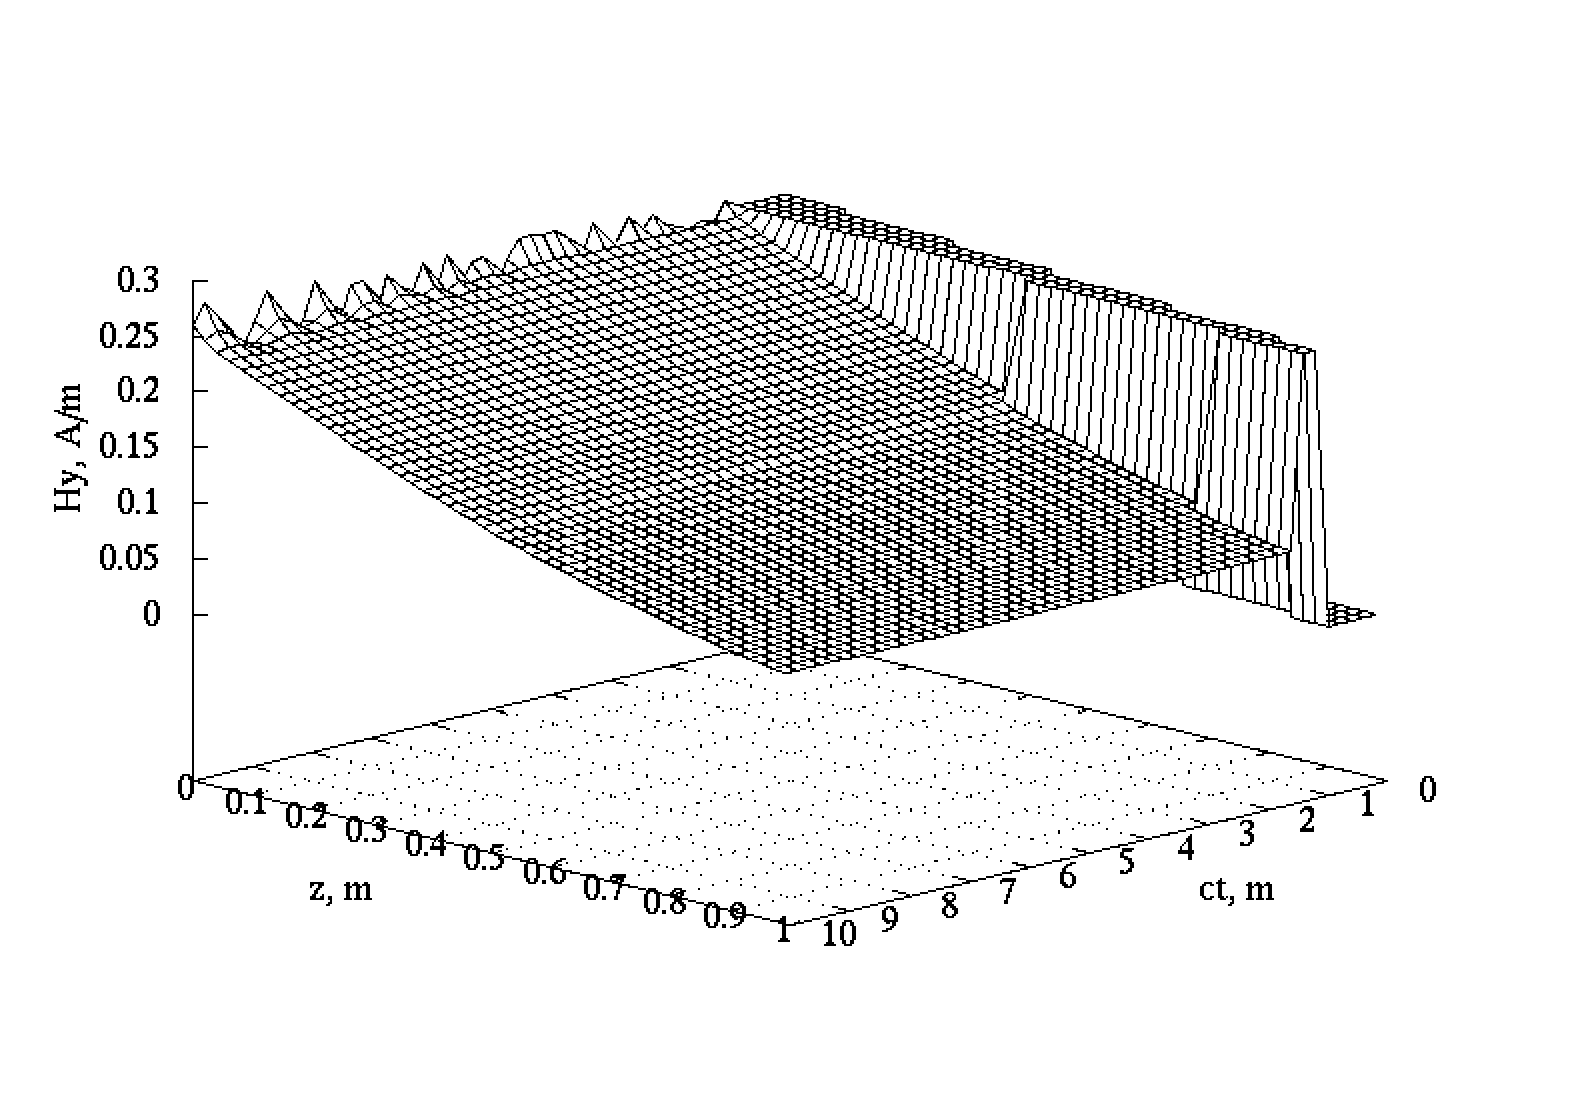
\includegraphics[scale=0.6]{StaticOnAxis}
\caption{Магнітно-статичне поле ($ \rho = 0 $ м)} \label{fig:emp_h_rho}
\end{center} \end{figure}
%
\begin{figure}[h] \begin{center}
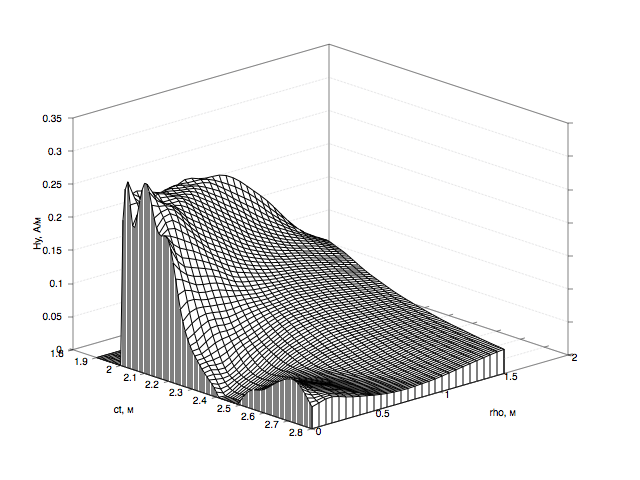
\includegraphics[scale=0.7]{LinearMagnetic}
\caption{Магнітно-статичне поле ($ z = 2 $ м)} \label{fig:emp_h_rho}
\end{center} \end{figure}

За визначенням дальньої зони - це область простору, де $ E_\varphi = H_\rho $ та
$ H_\varphi = E_\rho $. Дня лінійного поля плаского диску ці умови виконується, 
коли $ U_0(W_-,Z) - U_2(W_-,Z) = J_0(Z) $. Остання тотожність математично вірна
тоді і тільки коли 
%
\begin{equation} \label{eq:FraunhoferDistance}
\left. \lim_{z \to \infty} \left( \frac{ct-z}{ct+z} \right)^m 
\right|_{m > 1} = 0
\end{equation}

Остання тотожність є умовою дальньої зони для антени що породжує 
нестаціонарне поле. Варто зазначити, що при рості $ z $ росте і $ t $, 
відповідно до принципу причинності, тобто умова $ ct - z > 0 $ виконується.

%%%%%%%%%%%%%%%%%%%%%%%%%%%%%%%%%%%%%%%%%%%%%%%%%%%%%%%%%%%%%%%%%%%%%%%%%%%%%%%%
\section{Вторинне джерело поля в слабкому нелінійному середовищі. 
Нелінійність Керра}

При взаємодії з середовищем поле змінюється. Така повединка називається ефектом 
самодії. Джерелом такого поля стає весь простір його розповсюдження. Назвемо 
таке джерело вторинним. Випадки коли вторинним джерелом можна знехтувати, за 
рахунок його незначного вливу порівняно з первинним джерелом, називається 
лінійною задачею випромінювання. Прикладами такого поля є 
\eqref{eq:linear_h_cyl} та \eqref{eq:linear_e_cyl}. Тепер розглянемо 
середовище, де вплив самодії все ще незначний порівнянно з лінійним полем, але
викликає розбіжності в емпіричних показниках та данних теоретичної моделі. 
Таке середовище називають слабним нелінійним середовищем. Вторинне джерело 
поля в такому середовищі є функцією амплатуди поля. В якості такого джерела 
розглянемо вторинній електричний струм
%
\begin{equation*} 
\vect{J^\prime} = \partder{}{t} \vect{P^\prime} \left( \vect{E} \right)
\end{equation*}

Остання рівність складається з двох додаків. Перший додаток відповідає саме 
нелінійним властивостям поля. Останній додаток описує провідникові властивості 
середи розповлюдження, які теж мжуть бути описані вторинним джерелом. 
%
\begin{equation*} 
\vect{J^\prime} = 
\vect{\rho_0}    \partder{}{t} P_\rho^\prime    \left( \vect{E} \right) + 
\vect{\varphi_0} \partder{}{t} P_\varphi^\prime \left( \vect{E} \right) + 
\vect{z_0}       \partder{}{t} P_z^\prime       \left( \vect{E} \right) 
\end{equation*}
%
Вектор поляризвції для середовищі, де спостерігаюсься слабкі нелінійні ефкекти 
є довільною функцією, але може бути представлено в виді розкладу степеневого 
ряду Тейлора. 
%
\begin{equation*} \begin{aligned}
\vect{P^\prime} \left( \vect{E} \right) = \sum_{i=2}^{\infty} \xi_i \vect{E}^i
\end{aligned} \end{equation*}
%
Зауважимо, що розклад ведется по степеням вектора напружиності 
електричного поля, як у задачах оптики \textcolor{red}{[ПОСИЛАННЯ]}. 
Це створює математичні проблеми у доданках з парними коефіцієнтами.
вирішити їх можна домноженням на одиничний вектор.
%
\begin{equation*} \begin{aligned}
\vect{P^\prime}_2 \left( \vect{E} \right) = \xi_2 \vect{E}^2 = 
\xi_2 \vect{E}^2 \left( \vect{\rho_0}  + \vect{\varphi_0} + \vect{z_0} \right)
\end{aligned} \end{equation*}
%
\textcolor{red}{ Згідно з неоднозначностю векторного потенціалу 
\cite[ст. 77]{imp:LandauII} $ \vect{J^\prime} \left\{ S_1 \right\}  = 0 $. }
%
\textcolor{red}{ Чи правильно, що нелінійна ппроникність поля залежеть від 
амплтуди джерела? }
%
Для аналізу виберемо третій доданок неліної поляризації, який активно 
використовується в імпульсній електроніці \textcolor{red}{[ПОСИЛАННЯ]}.
%
\begin{equation*}
\vect{P^\prime} \left( \vect{E} \right) = 
\xi_3^e \vect{E}^3 
\left( A_0, R, \epsilon, \mu, vt, \vect{r} \right)
\end{equation*}
%
Під кубом вектора розуміється сам вектор домноженій на квадрат довжини.
\textcolor{red}{ Можливо, що природа нелінійних ефектів значно глибша і 
їх ефект впливає на характер енегетичної взаємодії та змінює простір.
Відповідно довжина вектора в декартовому сенсі втрачає змаст. }
%
\begin{equation*}
\vect{P^\prime} \left( \vect{E} \right) = 
\xi_3^e \dotprod{ \vect{E} }{ \vect{E} } \cdot \vect{E} 
\end{equation*}
%
В середовищі, де нелінійні ефекти описуються таким вектором
%
\textcolor{lightgray}{ \begin{equation*} \begin{aligned}
\vect{P^\prime} \left( \vect{E} \right) = 
\frac{ {A_0}^3 \xi_3^e }{ 8 } \left( \frac{\mu_0 \mu}
{\epsilon_0 \epsilon} \right)^{3/2} \left( {I_1}^2 \cos^2 \varphi + 
\left( I_2 - I_1 \right)^2 \sin^2 \varphi \right) \cdot \\ 
\cdot \Big( \vect{\rho_0} I_1 \cos \varphi - 
\vect{ \varphi_0 } \left( I_2 - I_1 \right) \sin \varphi \Big)
\end{aligned} \end{equation*} }
%
\textcolor{red}{ Які нелінійні ефекти спостерігаються в керрівському середовищі?}

%%%%%%%%%%%%%%%%%%%%%%%%%%%%%%%%%%%%%%%%%%%%%%%%%%%%%%%%%%%%%%%%%%%%%%%%%%%%%%%%
\section{Еволюційні коефіцієнти для нелінійної поправки до поля}
%
Для отримання нелінійної поправки до електричного поля спочатку отримаємо
розкладене по модовому базису вторинне джерело поля. Для цього, 
\textcolor{red}{згідно принципам віпромінювання}, знадобляться 
похідні компонентів електричного поля за часом. Часова залежність лінійного
електричного поля плаского дику міститься тільки в функціях 
$ I_1(ct,r) $ та $ I_2(ct,r) $. Для збереження безрозмарності розділимо
похідні на максимальну швидкість розповсюдженя для середовища.
%
\textcolor{lightgray}{ \begin{equation*} \begin{aligned}
I_1 \left\{ S_2 \right\} = \frac{\rho^2 + R^2}{4 \pi \rho^2} \arccos 
\frac{c^2 t^2 - z^2 - \rho^2 - R^2}{2 \rho R}  -
\frac{\sqrt{4 \rho^2 R^2 - (\rho^2 + R^2 - c^2t^2 + z^2)^2}}{4 \pi \rho^2} - \\
- \frac{ |\rho^2 - R^2| }{2 \pi \rho^2} 
\arctan \sqrt{ \frac{(\rho - R)^2}{(\rho + R)^2} \cdot
\frac{\left( \rho + R \right)^2 - \left( c^2t^2 - z^2 \right)} 
{\left( c^2t^2 - z^2 \right) - \left( \rho - R \right)^2} }
\end{aligned} \end{equation*} }
%
\textcolor{lightgray}{ \begin{equation*} \begin{aligned}
\partder{I_1 \left\{ S_2 \right\}}{t} = \frac{\rho^2 + R^2}{4 \pi \rho^2}
\partder{}{t} \arccos \frac{c^2 t^2 - z^2 - \rho^2 - R^2}{2 \rho R} - \\
- \partder{}{t} \frac{\sqrt{4 \rho^2 R^2 - (\rho^2 + R^2 - c^2t^2 + z^2)^2}}
{4 \pi \rho^2} - \\ - \frac{ |\rho^2 - R^2| }{2 \pi \rho^2} \partder{}{t} 
\arctan \sqrt{ \frac{(\rho - R)^2}{(\rho + R)^2} \cdot
\frac{\left( \rho + R \right)^2 - \left( c^2t^2 - z^2 \right)} 
{\left( c^2t^2 - z^2 \right) - \left( \rho - R \right)^2} }
\end{aligned} \end{equation*} }
%
\textcolor{lightgray}{ \begin{equation*} \begin{aligned}
\partder{}{t} \arccos \frac{c^2 t^2 - z^2 - \rho^2 - R^2}{2 \rho R} = 
- \frac{2 c^2 t}
{ \sqrt{4 \rho^2 R^2 - \left(c^2 t^2 - z^2 - \rho^2 - R^2 \right)^2} }
\end{aligned} \end{equation*} }
%
\textcolor{red}{ \begin{equation*} \begin{aligned}
- \partder{}{t} \left( \rho^2 + R^2 - c^2t^2 + z^2 \right)^2 = 
- 2 (\rho^2 + R^2 -c^2t^2 + z^2) (-2 c^2 t)
\end{aligned} \end{equation*} }
%
\textcolor{lightgray}{ \begin{equation*} \begin{aligned}
\partder{}{t} \frac{\sqrt{4 \rho^2 R^2 - (\rho^2 + R^2 - c^2t^2 + z^2)^2}}
{4 \pi \rho^2} = \frac{1}{8 \pi \rho^2} 
\frac{ 4 c^2 t (\rho^2 + R^2 - c^2 t^2 + z^2) }
{ \sqrt{4 \rho^2 R^2 - (\rho^2 + R^2 - c^2t^2 + z^2)^2} } = \\
= \frac{c^2 t}{2 \pi \rho^2} \frac{\rho^2 + R^2 - c^2 t^2 + z^2}
{ \sqrt{4 \rho^2 R^2 - (\rho^2 + R^2 - c^2t^2 + z^2)^2} }
\end{aligned} \end{equation*} }
%
\textcolor{red}{ \begin{equation*} \begin{aligned}
\partder{}{t} \arctan \sqrt{ \frac{x}{y} } = 
\frac{1}{1 + \frac{x}{y}} \frac{1}{2} 
\sqrt \frac{y}{x} \partder{}{t} \frac{x}{y}
\end{aligned} \end{equation*} }
%
\textcolor{red}{ \begin{equation*} \begin{aligned}
- \frac{1}{(\rho + R)^2} + \frac{1}{(\rho - R)^2} = 
\frac{- (\rho-R)^2 + (\rho+R)^2 }{ (\rho^2 - R^2)^2 }
\end{aligned} \end{equation*} }
%
\textcolor{lightgray}{ \begin{equation*} \begin{aligned}
\partder{}{t} \arctan \sqrt{ \frac{(\rho - R)^2}{(\rho + R)^2}
\frac{\left( \rho + R \right)^2 - \left( c^2t^2 - z^2 \right)} 
{\left( c^2t^2 - z^2 \right) - \left( \rho - R \right)^2} } = 
\partder{}{t} \arctan \sqrt{ \frac
{1 - \frac{c^2t^2 - z^2}{\left( \rho + R \right)^2} } 
{ \frac{c^2t^2 - z^2}{ \left( \rho - R \right)^2 } - 1} } = \\
= \frac{1}{1 + \frac{1 - \frac{c^2t^2 - z^2}{\left( \rho + R \right)^2} } 
{ \frac{c^2t^2 - z^2}{ \left( \rho - R \right)^2 } - 1} } \frac{1}{2}
\sqrt{ \frac{ \frac{c^2t^2 - z^2}{ \left( \rho - R \right)^2 } - 1 }
{1 - \frac{c^2t^2 - z^2}{\left( \rho + R \right)^2} } } 
\frac{ - \frac{2 c^2 t}{\left( \rho + R \right)^2} 
\left( \frac{c^2t^2 - z^2}{ \left( \rho - R \right)^2} - 1 \right) - 
\frac{ 2 c^2 t }{ \left( \rho - R \right)^2 } 
\left( 1 - \frac{c^2t^2 - z^2}{\left( \rho + R \right)^2} \right) }
{\left( \frac{c^2t^2 - z^2}{ \left( \rho - R \right)^2 } - 1 \right)^2} = \\
= - c^2 t \frac{ \frac{c^2t^2-z^2}{(\rho-R)^2} - 1 }
{ \frac{c^2t^2-z^2}{(\rho-R)^2} - 1 + 1 - 
\frac{c^2t^2 - z^2}{\left( \rho + R \right)^2} }
\sqrt{ \frac{ \frac{c^2t^2 - z^2}{ \left( \rho - R \right)^2 } - 1}
{1 - \frac{c^2t^2 - z^2}{\left( \rho + R \right)^2} } } \frac
{ \frac{c^2t^2 - z^2}{ \left( \rho^2 - R^2 \right)^2 } - \frac{1}{(\rho+R)^2} + 
\frac{1}{(\rho-R)^2} - \frac{ c^2t^2 - z^2 }{ \left( \rho^2 - R^2 \right)^2 } }
{ \left( \frac{c^2t^2 - z^2}{ \left( \rho - R \right)^2} - 1 \right)^2 } = \\
= - \frac{4 \rho R c^2 t}{ \left( \rho^2 - R^2 \right)^2 } 
\frac{ 1 }{ \frac{c^2t^2-z^2}{(\rho-R)^2} - 
\frac{c^2t^2 - z^2}{\left( \rho + R \right)^2} }
\sqrt{ \frac{ \frac{c^2t^2 - z^2}{ \left( \rho - R \right)^2 } - 1}
{1 - \frac{c^2t^2 - z^2}{\left( \rho + R \right)^2} } } \frac
{ 1 }{ \frac{c^2t^2 - z^2}{ \left( \rho - R \right)^2} - 1 } = \\
= - \frac{c^2 t}{ c^2 t^2 - z^2 } \frac{1} { 
\sqrt{ 1 - \frac{c^2t^2 - z^2}{(\rho + R)^2 } } 
\sqrt{ \frac{c^2t^2 - z^2}{ (\rho - R)^2 } - 1} }
\end{aligned} \end{equation*} }
%
\textcolor{lightgray}{ \begin{equation*} \begin{aligned}
\partder{ I_1 \{ S_2 \} }{t} = - \frac{c^2 t}{2 \pi \rho^2}
\frac{\rho^2 + R^2}
{ \sqrt{4 \rho^2 R^2 - \left(c^2 t^2 - z^2 - \rho^2 - R^2 \right)^2} } - \\
- \frac{c^2 t}{2 \pi \rho^2} \frac{\rho^2 + R^2 - c^2 t^2 + z^2}
{ \sqrt{4 \rho^2 R^2 - (\rho^2 + R^2 - c^2t^2 + z^2)^2} } + \\ 
+ \frac{ c^2 t }{2 \pi \rho^2} \frac{|\rho^2 - R^2|}{ c^2 t^2 - z^2 } \frac{1} 
{ \sqrt{ 1 - \frac{c^2t^2 - z^2}{(\rho + R)^2 } } 
\sqrt{ \frac{c^2t^2 - z^2}{ (\rho - R)^2 } - 1} }
\end{aligned} \end{equation*} }
%
\begin{equation*} \begin{aligned}
\frac{1}{c} \partder{ I_1 \{ S_2 \} }{t} = \frac{ ct }{2 \pi \rho^2} 
\frac{ (\rho^2 - R^2)^2  (c^2 t^2 - z^2)^{-1} } 
{ \sqrt{ (\rho + R)^2 - c^2t^2 + z^2 } 
\sqrt{ c^2t^2 - z^2 - (\rho - R)^2 } } - \\
- \frac{ct}{2 \pi \rho^2} \frac{2 (\rho^2 + R^2) - (c^2 t^2 - z^2)}
{ \sqrt{4 \rho^2 R^2 - (c^2t^2 - z^2 - \rho^2 - R^2)^2} }
\end{aligned} \end{equation*}
%
\begin{equation*} \begin{aligned}
\frac{1}{c} \partder{ I_1 \{ S_{1,3} \} }{t} = 0
\end{aligned} \end{equation*}
%
\textcolor{lightgray}{ \begin{equation*} \begin{aligned}
\partder{ I_2 \{ S_2 \} }{t} = \frac{1}{\pi} \partder{}{t} \arccos 
\frac{c^2t^2 - z^2 + \rho^2 - R^2}{2 \rho \sqrt{c^2t^2 - z^2}} = \\
= - \frac{1}{\pi} \frac{1} { \sqrt{ 1 - \frac{ (c^2t^2 - z^2 + \rho^2 - R^2)^2 }
{4 \rho^2 (c^2t^2 - z^2)^2} } } \frac{1}{2 \rho} \partder{}{t} 
\frac{c^2t^2 - z^2 + \rho^2 - R^2} {\sqrt{c^2t^2 - z^2}} = \\
= - \frac{1}{2 \rho \pi} \frac{1} 
{ \sqrt{ 1 - \frac{ (c^2t^2 - z^2 + \rho^2 - R^2)^2 }
{4 \rho^2 (c^2t^2 - z^2)} } } \frac{2c^2t \sqrt{c^2t^2 - z^2} - 
\frac{c^2t}{\sqrt{c^2t^2 - z^2}} (c^2t^2 - z^2 + \rho^2 - R^2)
}{c^2t^2 - z^2} = \\ = - \frac{c^2 t}{2 \pi \rho} \frac{1} 
{ \sqrt{ 1 - \frac{ (c^2t^2 - z^2 + \rho^2 - R^2)^2 }
{4 \rho^2 (c^2t^2 - z^2)} } } \frac{2 \sqrt{c^2t^2 - z^2} - 
\frac{c^2t^2 - z^2 + \rho^2 - R^2}{\sqrt{c^2t^2 - z^2}}}{c^2t^2 - z^2} = \\
= - \frac{c^2 t}{2 \pi \rho (c^2t^2 - z^2)} \frac{ 2 \sqrt{c^2t^2 - z^2} - 
\frac{c^2t^2 - z^2 + \rho^2 - R^2}{\sqrt{c^2t^2 - z^2}} } 
{ \sqrt{ 1 - \frac{ (c^2t^2 - z^2 + \rho^2 - R^2)^2 }
{4 \rho^2 (c^2t^2 - z^2)} } } = \\
= - \frac{c^2 t}{\pi (c^2t^2 - z^2) } 
\frac{ 2 (c^2t^2 - z^2) - (c^2t^2 - z^2 + \rho^2 - R^2) } 
{ \sqrt{ 4 \rho^2 (c^2t^2 - z^2) - (c^2t^2 - z^2 + \rho^2 - R^2)^2 } } = \\
= - \frac{c^2 t}{\pi (c^2t^2 - z^2) } \frac{ c^2t^2 - z^2 -  \rho^2 + R^2 } 
{ \sqrt{ 4 \rho^2 (c^2t^2 - z^2) - (c^2t^2 - z^2 + \rho^2 - R^2)^2 } }
\end{aligned} \end{equation*} }
%
\begin{equation*} \begin{aligned}
\frac{1}{c} \partder{ I_2 \{ S_2 \} }{t} = 
- \frac{ct}{\pi (c^2t^2 - z^2) } \frac{ c^2t^2 - z^2 -  \rho^2 + R^2 } 
{ \sqrt{ 4 \rho^2 (c^2t^2 - z^2) - (c^2t^2 - z^2 + \rho^2 - R^2)^2 } }
\end{aligned} \end{equation*}
%
\begin{equation*} \begin{aligned}
\frac{1}{c} \partder{ I_2 \{ S_{1,3} \} }{t} = 0
\end{aligned} \end{equation*}
%
Тепер запишемо компоненти електричного струму, який є вторинним джерелом
електромагнітного поля. З компонентою $ \vect{z_0} $ все просто - 
поздовжне електричне поле дорівнює нулю.
%
\textcolor{lightgray}{ \begin{equation*} \begin{aligned}
\vect{P^\prime} \left( \vect{E} \right) = 
\frac{ {A_0}^3 \xi_3 }{ 8 } \left( \frac{\mu_0 \mu}
{\epsilon_0 \epsilon} \right)^{3/2} \left( {I_1}^2 \cos^2 \varphi + 
\left( I_2 - I_1 \right)^2 \sin^2 \varphi \right) \cdot \\ 
\cdot \Big( \vect{\rho_0} I_1 \cos \varphi - 
\vect{ \varphi_0 } \left( I_2 - I_1 \right) \sin \varphi \Big)
\end{aligned} \end{equation*} }
%
\textcolor{lightgray}{ \begin{equation*} \label{eq:linear_e_cyl}
\vect{E} = \frac{A_0}{2} \sqrt{\frac{\mu_0 \mu}{\epsilon_0 \epsilon}}
\Big( \vect{\rho_0} I_1 \cos \varphi - 
\vect{ \varphi_0 } \left( I_2 - I_1 \right) \sin \varphi \Big)
\end{equation*} }
%
\textcolor{lightgray}{ \begin{equation*} \begin{aligned}
\vect{E}^2 = \frac{A_0^2}{4} \frac{\mu_0 \mu}{\epsilon_0 \epsilon}
\Big( I_1^2 \cos^2 \varphi + \left( I_2 - I_1 \right)^2 \sin^2 \varphi \Big)
\end{aligned} \end{equation*} }
%
\textcolor{lightgray}{ \begin{equation*} \begin{aligned}
\partder{ \vect{E}^2 }{t} = \frac{A_0^2}{4} 
\frac{\mu_0 \mu}{\epsilon_0 \epsilon}
\left( 2 I_1 \partder{I_1}{t} \cos^2 \varphi + 
2 ( I_2 - I_1 ) \left( \partder{I_2}{t} - \partder{I_1}{t} \right) 
\sin^2 \varphi \right)
\end{aligned} \end{equation*} }
%
\begin{equation*} \begin{aligned}
\partder{P_z^\prim}{t} = 0
\end{aligned} \end{equation*}
%
Вирази для поперечних компонентів поля стають шматочновизначиними,
через свої залежності.
%
\textcolor{lightgray} { \begin{equation*} \begin{aligned}
\partder{P_\rho^\prime}{t}   = \frac{ {A_0}^3 \xi_3 }{ 8 } 
\left( \frac{\mu_0 \mu} {\epsilon_0 \epsilon} \right)^{3/2} \left(
\left( {I_1}^2 \cos^2 \varphi + ( I_2 - I_1 )^2 \sin^2 \varphi \right)
\partder{I_1}{t} \cos \varphi + \right. \\
\left. + I_1 \cos \varphi \left( 2 I_1 \partder{I_1}{t} \cos^2 \varphi + 
2 ( I_2 - I_1 ) \left( \partder{I_2}{t} - \partder{I_1}{t} \right) 
\sin^2 \varphi \right) \right) = \\ = \frac{ {A_0}^3 \xi_3^e }{ 8 } 
\left( \frac{\mu_0 \mu} {\epsilon_0 \epsilon} \right)^{3/2} \left(
\partder{I_1}{t} {I_1}^2 \cos^3 \varphi + \partder{I_1}{t} ( I_2 - I_1 )^2 
\cos \varphi \sin^2 \varphi + \right. \\
\left. + 2 {I_1}^2 \partder{I_1}{t} \cos^3 \varphi + 
2 I_1 ( I_2 - I_1 ) \left( \partder{I_2}{t} - \partder{I_1}{t} \right) 
\cos \varphi \sin^2 \varphi \right)
\end{aligned} \end{equation*} }
%
\begin{equation*} \begin{aligned}
\partder{P_\rho^\prime}{t} = \frac{ {A_0}^3 \xi_3 }{ 8 } 
\left( \frac{\mu_0 \mu} {\epsilon_0 \epsilon} \right)^{3/2} \left(
3 {I_1}^2 \partder{I_1}{t} \cos^3 \varphi + \right. \\
+ \left. ( I_2 - I_1 ) \cos \varphi \sin^2 \varphi \left( 
\partder{I_1}{t} ( I_2 - I_1 ) + 2 I_1 \left( \partder{I_2}{t} - 
\partder{I_1}{t} \right) \right) \right)
\end{aligned} \end{equation*}
%
\textcolor{lightgray} { \begin{equation*} \begin{aligned}
\partder{P_\varphi^\prime}{t}   = - \frac{ {A_0}^3 \xi_3 }{ 8 } 
\left( \frac{\mu_0 \mu} {\epsilon_0 \epsilon} \right)^{3/2} \left(
\left( {I_1}^2 \cos^2 \varphi + ( I_2 - I_1 )^2 \sin^2 \varphi \right)
\left( \partder{I_2}{t} - \partder{I_1}{t} \right) \sin \varphi + \right. \\
\left. + (I_2 - I_1) \sin \varphi \left( 2 I_1 \partder{I_1}{t} \cos^2 \varphi + 
2 ( I_2 - I_1 ) \left( \partder{I_2}{t} - \partder{I_1}{t} \right) 
\sin^2 \varphi \right) \right) = \\ = - \frac{ {A_0}^3 \xi_3 }{ 8 } 
\left( \frac{\mu_0 \mu} {\epsilon_0 \epsilon} \right)^{3/2} \left(
{I_1}^2 \left( \partder{I_2}{t} - \partder{I_1}{t} \right) 
\sin \varphi \cos^2 \varphi + \right. \\ \left. 
+ ( I_2 - I_1 )^2 \left( \partder{I_2}{t} - \partder{I_1}{t} \right) 
\sin^3 \varphi + 2 I_1 \partder{I_1}{t} (I_2 - I_1) 
\sin \varphi \cos^2 \varphi + \right. \\ 
+ \left. 2 ( I_2 - I_1 )^2 \left( \partder{I_2}{t} - \partder{I_1}{t} \right) 
\sin^3 \varphi \right)
\end{aligned} \end{equation*} }
%
\begin{equation*} \begin{aligned}
\partder{P_\varphi^\prime}{t} = - \frac{ {A_0}^3 \xi_3 }{ 8 } 
\left( \frac{\mu_0 \mu} {\epsilon_0 \epsilon} \right)^{3/2} \left(
3 ( I_2 - I_1 )^2 \left( \partder{I_2}{t} - \partder{I_1}{t} \right)
\sin^3 \varphi \right. + \\
+ \left. I_1 \sin \varphi \cos^2 \varphi \left( 
I_1 \left( \partder{I_2}{t} - \partder{I_1}{t} \right) + 
2 \partder{I_1}{t} (I_2 - I_1) \right) \right)
\end{aligned} \end{equation*}
%
Для запису модового струму використаємо формулу ..., що 
є кратиним інтегралом по точкам випромінювання та має комплексну
область значень.
%
\textcolor{lightgray} { \begin{equation*}
j_m \left( r, t; \nu \right) = \frac{\sqrt{\mu_0}}{2\pi} 
\int \limits_{0}^{2\pi} d \varphi \int \limits_0^\infty \rho d \rho 
\vect{j_0} \crossprod{ \nabla_\perp \Psi_m^* }{ \vect{z_0} }
\end{equation*} }
%
\textcolor{lightgray} { \begin{equation*} 
\vect{J^\prime} = 
\vect{\rho_0}    \partder{}{t} P_\rho^\prime    \left( \vect{E} \right) + 
\vect{\varphi_0} \partder{}{t} P_\varphi^\prime \left( \vect{E} \right) + 
\vect{z_0}       \partder{}{t} P_z^\prime       \left( \vect{E} \right) 
\end{equation*} }
%
\textcolor{lightgray} { \begin{equation*} \begin{aligned}
\crossprod{ \nabla_\perp \Psi_m^* }{ \vect{z_0} } =
- \vect{\rho_0} i m e^{-im\varphi} \frac{J_m (\nu \rho)}{\rho \sqrt{\nu}}
- \vect{\varphi_0} \sqrt{\nu} e^{-im\varphi} 
\frac{J_{m-1} (\nu \rho) - J_{m+1} (\nu \rho)}{2}
\end{aligned} \end{equation*} }
%
\textcolor{lightgray} { \begin{equation*} \begin{aligned}
\vect{J^\prime} \crossprod{ \nabla_\perp \Psi_m^* }{ \vect{z_0} } = 
- i e^{-im\varphi} m \frac{J_m (\nu \rho)}{\rho \sqrt{\nu}}
\partder{}{t} P_\rho^\prime \left( \vect{E} \right) - \\
- \sqrt{\nu} e^{-im\varphi} \frac{J_{m-1} (\nu \rho) - J_{m+1} (\nu \rho)}{2}
\partder{}{t} P_\varphi^\prime \right)
\end{aligned} \end{equation*} }
%
\begin{equation*} \begin{aligned}
j_m = - \frac{\sqrt{\mu_0}}{2\pi} 
\int_{0}^{2\pi} d \varphi \int \limits_{0}^{\infty} \rho d \rho
e^{-im\varphi} \left( i  m \frac{J_m (\nu \rho)}{\rho \sqrt{\nu}}
\partder{P_\rho^\prime}{t} + \sqrt{\nu}
\frac{J_{m-1} (\nu \rho) - J_{m+1} (\nu \rho)}{2}
\partder{P_\varphi^\prime}{t} \right)
\end{aligned} \end{equation*}
%
Згрупувавши доданки за тригонометричними функціями, що вони містять,
знайдемо інтеграли за зменним азимутальним кутом $ \varphi $. Самі інеграли
взяті окремо в додатку ..., випишимо лише результати.
%
\textcolor{lightgray} { \begin{equation*} \begin{aligned}
\int_{0}^{2 \pi} d \varphi e^{-im \varphi} \partder{P_\rho^\prime}{t} = 
\frac{ {A_0}^3 \xi_3 }{ 8 } \int_{0}^{2\pi} d \varphi
e^{-im\varphi} \left( \frac{\mu_0 \mu} {\epsilon_0 \epsilon} \right)^{3/2} 
\left( 3 {I_1}^2 \partder{I_1}{t} \cos^3 \varphi + \right. \\
+ \left. ( I_2 - I_1 ) \cos \varphi \sin^2 \varphi \left( 
\partder{I_1}{t} ( I_2 - I_1 ) + 2 I_1 \left( \partder{I_2}{t} - 
\partder{I_1}{t} \right) \right) \right) = \\
= \frac{ {A_0}^3 \xi_3 }{ 8 } 
\left( \frac{\mu_0 \mu} {\epsilon_0 \epsilon} \right)^{3/2}
\left( \frac{3 \pi}{4} {I_1}^2 \partder{I_1}{t} \left( \delta_{m,-3} - 
\delta_{m,3} + 3 \delta_{m,-1} + 3 \delta_{m,1} \right) + \right. \\
+ \frac{\pi }{4} \left. ( I_2 - I_1 ) \left( \delta_{m,1} - 
\delta_{m,-3} + \delta_{m,-1} - \delta_{m,3} \right) \left( 
\partder{I_1}{t} ( I_2 - I_1 ) + 2 I_1 \left( \partder{I_2}{t} - 
\partder{I_1}{t} \right) \right) \right)
\end{aligned} \end{equation*} }
%
\textcolor{lightgray} { \begin{equation*} \begin{aligned}
\int_{0}^{2\pi} e^{-i m \varphi} \cos^3 \varphi d \varphi = 
\frac{\pi}{4} \delta_{m,-3} - \frac{\pi}{4} \delta_{m,3} + 
\frac{3 \pi}{4} \delta_{m,-1} + \frac{3 \pi}{4} \delta_{m,1}
\end{aligned} \end{equation*} }
%
\textcolor{lightgray} { \begin{equation*} \begin{aligned}
\int_{0}^{2\pi} e^{-i m \varphi} \cos \varphi \sin^2 \varphi d \varphi = 
\frac{\pi \delta_{m,1} }{4} - \frac{\pi \delta_{m,-3} }{4} + 
\frac{\pi \delta_{m,-1} }{4} - \frac{\pi \delta_{m,3} }{4}
\end{aligned} \end{equation*} }
%
\begin{equation*} \begin{aligned}
\int_{0}^{2\pi} d \varphi e^{-im \varphi} \partder{P_\rho^\prime}{t} = 
\frac{ {A_0}^3 \xi_3 \pi }{ 4 \cdot 8 } 
\left( \frac{\mu_0 \mu} {\epsilon_0 \epsilon} \right)^{3/2}
\left( 3 {I_1}^2 \partder{I_1}{t} \left( \delta_{m,-3} - 
\delta_{m,3} + 3 \delta_{m,-1} + 3 \delta_{m,1} \right) + \right. \\
+ \left. ( I_2 - I_1 ) \left( \delta_{m,1} - 
\delta_{m,-3} + \delta_{m,-1} - \delta_{m,3} \right) \left( 
\partder{I_1}{t} ( I_2 - I_1 ) + 2 I_1 \left( \partder{I_2}{t} - 
\partder{I_1}{t} \right) \right) \right)
\end{aligned} \end{equation*}
%
\textcolor{lightgray} { \begin{equation*} \begin{aligned}
\int_{0}^{2\pi} e^{-i m \varphi} \sin^3 \varphi d \varphi = 
\frac{3 \pi i}{4} \delta_{m,-1} - \frac{3 \pi i}{4} \delta_{m,1} - 
\frac{\pi i}{4} \delta_{m,-3} - \frac{\pi i}{4} \delta_{m,3}
\end{aligned} \end{equation*} }
%
\textcolor{lightgray} { \begin{equation*} \begin{aligned}
\int_{0}^{2\pi} e^{-i m \varphi} \sin \varphi \cos^2 \varphi d \varphi = 
\frac{\pi i }{4} \delta_{m,-3} - \frac{\pi i }{4} \delta_{m,1} + 
\frac{\pi i }{4} \delta_{m,3} + \frac{\pi i }{4} \delta_{m,-1}
\end{aligned} \end{equation*} }
%
\textcolor{lightgray} { \begin{equation*} \begin{aligned}
\int_{0}^{2 \pi} d \varphi e^{-im \varphi} \partder{P_\varphi^\prime}{t} = \\
= - \frac{ {A_0}^3 \xi_3 }{ 8 } \int_{0}^{2 \pi} d \varphi e^{-im \varphi}
\left( \frac{\mu_0 \mu} {\epsilon_0 \epsilon} \right)^{3/2} \left(
3 ( I_2 - I_1 )^2 \left( \partder{I_2}{t} - \partder{I_1}{t} \right)
\sin^3 \varphi \right. + \\
+ \left. I_1 \sin \varphi \cos^2 \varphi \left( 
I_1 \left( \partder{I_2}{t} - \partder{I_1}{t} \right) + 
2 \partder{I_1}{t} (I_2 - I_1) \right) \right) = 
- \frac{ {A_0}^3 \xi_3 }{ 8 V } \cdot \\ 
\cdot \left( \frac{\mu_0 \mu} {\epsilon_0 \epsilon} \right)^{3/2} \left(
\frac{3 \pi i}{4} ( I_2 - I_1 )^2 \left( \partder{I_2}{t} - 
\partder{I_1}{t} \right) \left( 3 \delta_{m,-1} - 3 \delta_{m,1} - 
\delta_{m,-3} - \delta_{m,3} \right) \right. + \\
+ \left. \frac{\pi i}{4} I_1 \left(  \delta_{m,-3} - \delta_{m,1} + 
\delta_{m,3} + \delta_{m,-1} \right) \left( 
I_1 \left( \partder{I_2}{t} - \partder{I_1}{t} \right) + 
2 \partder{I_1}{t} (I_2 - I_1) \right) \right)
\end{aligned} \end{equation*} }
%
\begin{equation*} \begin{aligned}
\int_{0}^{2 \pi} d \varphi e^{-im \varphi} \partder{P_\varphi^\prime}{t} = 
- \frac{ {A_0}^3 \xi_3  i \pi }{ 4 \cdot 8 }
\left( \frac{\mu_0 \mu} {\epsilon_0 \epsilon} \right)^{3/2} \cdot \\ 
\cdot \left( 3 ( I_2 - I_1 )^2 \left( \partder{I_2}{t} - 
\partder{I_1}{t} \right) \left( 3 \delta_{m,-1} - 3 \delta_{m,1} - 
\delta_{m,-3} - \delta_{m,3} \right) \right. + \\
+ \left. I_1 \left(  \delta_{m,-3} - \delta_{m,1} + 
\delta_{m,3} + \delta_{m,-1} \right) \left( 
I_1 \left( \partder{I_2}{t} - \partder{I_1}{t} \right) + 
2 \partder{I_1}{t} (I_2 - I_1) \right) \right)
\end{aligned} \end{equation*}
%
\textcolor{lightgray} { \begin{equation*} \begin{aligned}
\int \limits_{0}^{2\pi} d \varphi \sin \varphi 
\left( \cos m \varphi - i \sin m \varphi \right) = 
i \pi \left( \delta_{m,-1} - \delta_{m,1} \right)
\end{aligned} \end{equation*} }
%
\textcolor{lightgray} { \begin{equation*} \begin{aligned}
\int \limits_{0}^{2\pi} d \varphi \cos \varphi 
( \cos m \varphi - i \sin m \varphi) = \pi ( \delta_{m,-1} + \delta_{m,1} )
\end{aligned} \end{equation*} }
%
Тепер введемо нові змінні для того, щоб записати струм в визначенні модового 
базису, як інтеграл за радиалькою координатою $ \rho $. Тут з'являються змінні
за штрихованими кординатами. Так ми означимо кординати джерела випромінювання,
щоб уникнути плутанини з кординатами точки спостереження. Нехай ...
%
\textcolor{lightgray} { \begin{equation*} \begin{aligned}
N_1 (m) =  \frac{3 m {A_0}^3 \xi_3 \sqrt{\mu_0}}{64 \sqrt{\nu}} \frac{\pi}{\pi}
\left( \frac{\mu_0 \mu} {\epsilon_0 \epsilon} \right)^{3/2} 
\int_{0}^{\infty} d \rho 
J_m (\nu \rho) {I_1}^2 \partder{I_1}{t}
\end{aligned} \end{equation*} }
%
\textcolor{lightgray} { \begin{equation*} \begin{aligned}
N_1 (m) =  3 m J_m (\nu \rho) {I_1}^2 \partder{I_1}{t}
\end{aligned} \end{equation*} }
%
\begin{equation*} \begin{aligned}
N_1 (m) =  3 m J_m (\nu \rho') {I_1}^2 \partder{I_1}{t'}
\end{aligned} \end{equation*}
%
\textcolor{lightgray} { \begin{equation*} \begin{aligned}
N_2 (m) = \frac{m {A_0}^3 \xi_3 \sqrt{\mu_0}}{64 \sqrt{\nu}} \frac{\pi}{\pi}
\left( \frac{\mu_0 \mu} {\epsilon_0 \epsilon} \right)^{3/2} 
\int_{0}^{\infty} d \rho \\
J_m (\nu \rho) (I_2 - I_1) \left( \partder{I_1}{t} (I_2 - I_1) + 
2 I_1 \left( \partder{I_2}{t} - \partder{I_1}{t} \right) \right)
\end{aligned} \end{equation*} }
%
\textcolor{lightgray} { \begin{equation*} \begin{aligned}
N_2 (m) = m J_m (\nu \rho) (I_2 - I_1) \left( \partder{I_1}{t} (I_2 - I_1) + 
2 I_1 \left( \partder{I_2}{t} - \partder{I_1}{t} \right) \right)
\end{aligned} \end{equation*} }
%
\begin{equation*} \begin{aligned}
N_2 (m) = m J_m (\nu \rho') (I_2 - I_1) \left( \partder{I_1}{t'} (I_2 - I_1) + 
2 I_1 \left( \partder{I_2}{t'} - \partder{I_1}{t'} \right) \right)
\end{aligned} \end{equation*}
%
\textcolor{lightgray} { \begin{equation*} \begin{aligned}
N_3 (m) = - \frac{3 {A_0}^3 \xi_3 \sqrt{\mu_0}}{64} \sqrt{\nu} \frac{\pi}{\pi}
\left( \frac{\mu_0 \mu} {\epsilon_0 \epsilon} \right)^{3/2} 
\int_{0}^{\infty} \rho d \rho 
\frac{J_{m-1} (\nu \rho) - J_{m+1} (\nu \rho)}{2} \\
(I_2 - I_1)^2 \left( \partder{I_2}{t} - \partder{I_1}{t} \right) 
\end{aligned} \end{equation*} }
%
\textcolor{lightgray} { \begin{equation*} \begin{aligned}
N_3 (m) = - 3 \nu \rho
\frac{J_{m-1} (\nu \rho) - J_{m+1} (\nu \rho)}{2}
(I_2 - I_1)^2 \left( \partder{I_2}{t} - \partder{I_1}{t} \right)
\end{aligned} \end{equation*} }
%
\begin{equation*} \begin{aligned}
N_3 (m) = - 3 \nu \rho'
\frac{J_{m-1} (\nu \rho') - J_{m+1} (\nu \rho')}{2}
(I_2 - I_1)^2 \left( \partder{I_2}{t'} - \partder{I_1}{t'} \right)
\end{aligned} \end{equation*}
%
\textcolor{lightgray} { \begin{equation*} \begin{aligned}
N_4 (m) = - \frac{ {A_0}^3 \xi_3 \sqrt{\mu_0}}{64} \sqrt{\nu} \frac{\pi}{\pi}
\left( \frac{\mu_0 \mu} {\epsilon_0 \epsilon} \right)^{3/2}
\int_{0}^{\infty} \rho d \rho 
\frac{J_{m-1} (\nu \rho) - J_{m+1} (\nu \rho)}{2} \\
I_1 \left( I_1 \left( \partder{I_2}{t} - \partder{I_1}{t} \right) + 
2 \partder{I_1}{t} \left( I_2 - I_1 \right) \right)
\end{aligned} \end{equation*} }
%
\textcolor{lightgray} { \begin{equation*} \begin{aligned}
N_4 (m) = - \nu \rho
\frac{J_{m-1} (\nu \rho) - J_{m+1} (\nu \rho)}{2}
\left( I_1 \left( \partder{I_2}{t} - \partder{I_1}{t} \right) + 
2 \partder{I_1}{t} \left( I_2 - I_1 \right) \right)
\end{aligned} \end{equation*} }
%
\begin{equation*} \begin{aligned}
N_4 (m) = - \nu \rho'
\frac{J_{m-1} (\nu \rho') - J_{m+1} (\nu \rho')}{2} I_1
\left( I_1 \left( \partder{I_2}{t'} - \partder{I_1}{t'} \right) + 
2 \partder{I_1}{t'} \left( I_2 - I_1 \right) \right)
\end{aligned} \end{equation*}
%
Тоді їх сумми для кожної з кутових мод матимуть наступний вигляд. 
%
\textcolor{lightgray} { \begin{equation*} \begin{aligned}
N_{-1}^{sum} =  i \delta_{m,-1} \left( 3 N_1 (m) + N_2 (m) + 
3 N_3 (m) + N_4 (m) \right)
\end{aligned} \end{equation*} }
%
\begin{equation*} \begin{aligned}
N_{-1}^{sum} = 3 N_1 (-1) + N_2 (-1) + 3 N_3 (-1) + N_4 (-1)
\end{aligned} \end{equation*}
%
\textcolor{lightgray} { \begin{equation*} \begin{aligned}
N_{1}^{sum} =  i \delta_{m,1} \left( 3 N_1 (m) + N_2 (m) - 
3 N_3 (m) - N_4 (m) ) \right)
\end{aligned} \end{equation*} }
%
\begin{equation*} \begin{aligned}
N_{1}^{sum} = 3 N_1 (1) + N_2 (1) - 3 N_3 (1) - N_4 (1)
\end{aligned} \end{equation*}
%
\textcolor{lightgray} { \begin{equation*} \begin{aligned}
N_{-3}^{sum} =  i \delta_{m,-3} \left( N_1 (m) - N_2 (m) - 
N_3 (m) + N_4 (m) \right)
\end{aligned} \end{equation*} }
%
\begin{equation*} \begin{aligned}
N_{-3}^{sum} = N_1 (-3) - N_2 (-3) - N_3 (-3) + N_4 (-3)
\end{aligned} \end{equation*}
%
\textcolor{lightgray} { \begin{equation*} \begin{aligned}
N_{3}^{sum} =  i \delta_{m,3} \left( - N_1 (m) - N_2 (m) - 
N_3 (m) + N_4 (m) \right)
\end{aligned} \end{equation*} }
%
\begin{equation*} \begin{aligned}
N_{3}^{sum} = - N_1 (3) - N_2 (3) - N_3 (3) + N_4 (3)
\end{aligned} \end{equation*}
%
Тепер запишимо модовий струм в нових зменних.
%
\begin{equation*} \begin{aligned}
j'_m (t',z') = - \frac{i \xi_3 A_0^3 \sqrt{\mu_0}}{64 \sqrt{\nu}}
\left( \frac{\mu_0 \mu} {\epsilon_0 \epsilon} \right)^{3/2}
\int_{0}^{\infty} N_{m}^{sum} (\rho',t',z') d \rho'
\end{aligned} \end{equation*}
%
Помічаємо деякі властивості нових змінних $ N_i(m) $
%
\textcolor{red} { \begin{equation*} \begin{aligned}
N_{-m} = N_{m}
\end{aligned} \end{equation*}  }
%
А також та $ N_i^{sum} $
%
\textcolor{red} { \begin{equation*} \begin{aligned}
N_{-m}^{sum} = N_{m}^{sum}
\end{aligned} \end{equation*}  }

%%%%%%%%%%%%%%%%%%%%%%%%%%%%%%%%%%%%%%%%%%%%%%%%%%%%%%%%%%%%%%%%%%%%%%%%%%%%%%%%
\section{Нелінійна поправка}
%
Тепер коли визначено джерело можна застосувати метод еволюційних рівнянь.
Почнемо з розв'язку рівняння Клейна-Гордона.
%
\begin{equation*}
\frac{\epsilon \mu}{ \sqrt{\epsilon_0 \mu_0}} 
\frac{\partial^2 h_m}{\partial t^2} - \frac{\partial^2 h_m}{\partial z^2} + 
\nu^2 h_m = j_m (t',z'; \nu)
\end{equation*}
%
Коефіцієнт $ h_m $ доведеться розраховувати чисельно за формолою
%
\begin{equation*}
h_m (z, t; \nu) = \int_{0}^{\infty} \int_{0}^{\infty}
j_m (t',z'; \nu) G(t,t',z,z') dz' dt'
\end{equation*}
%
де 
%
\begin{equation*}
G(t,t',z,z') = \frac{\mathit{V}}{2} H \left( \mathit{V} (t-t') - (z-z') \right)
J_0 \left( \nu \sqrt{\mathit{V}^2 (t-t')^2 - (z-z')^2} \right)
\end{equation*}
%
З $ h_m $ можна отримати інші магнітні коефіцієнти
%
\begin{equation*}
I_m^h = \partial_z (h_m)
\end{equation*}
%
\begin{equation*}
V_m^h = - \mu \partial_{ct} (h_m)
\end{equation*}
%
Аналогічно для продольного коєфіціенту електричного поля
%
\textcolor{lightgray}{ \begin{equation*}
- \partial_{ct}(\mu I_n^e) - \partial_z V_n^e + \chi^2 e_n = 0
\end{equation*} }
%
\textcolor{lightgray}{ \begin{equation*}
\epsilon \mu \partial_{ct} \left( \partial_{ct} e_n + 
\frac{\sqrt{\mu_0}}{2 \pi} \int_0^{2\pi} d \varphi 
\int_0^{\infty} \rho d \rho \Phi_n^* (\chi) J_z \right) - 
\partial^2_z e_n + \chi^2 e_n = 0
\end{equation*} }
%
\begin{equation*}
\frac{\epsilon \mu}{ \sqrt{\epsilon_0 \mu_0}} 
\frac{\partial^2 e_n}{\partial t^2} - 
\frac{\partial^2 e_n}{\partial z^2} + \chi^2 e_n = 
- \frac{\sqrt{\mu_0}}{2 \pi c} 
\int_0^{2\pi} d \varphi 
\int_0^{\infty} \rho d \rho \Phi_n^* (\chi) \partder{J_z}{t}
\end{equation*}
%
Поздовжний вторинний електричний струм рівний нулю, тому рівняння 
Клейна-Гордона для $ e_n (z, t; \chi) $ є однорідним та має нульовий розвязок.
%
\begin{equation*}
e_n (z, t; \chi) = \iint_S j_n (t',z', \chi) G(t,t',z,z') dt' dz' = 0
\end{equation*}
%
Також чисельно знайдемо розвязки еволюційних рівнянь, що залишились.
%
\textcolor{lightgray}{ \begin{equation*}
\partial_{ct} (\epsilon e_n) = - I_n^e - 
\frac{\sqrt{\mu_0}}{2 \pi} \int_0^{2\pi} d \varphi 
\int_0^{\infty} \rho d \rho \Phi_n^* (\chi) J_z
\end{equation*} }
%
\begin{equation*}
I_n^e = - \partial_{ct} (\epsilon e_n) - 
\frac{\sqrt{\mu_0}}{2 \pi} \int_0^{2\pi} d \varphi 
\int_0^{\infty} \rho d \rho \Phi_n^* (\chi) J_z
\end{equation*}
%
\begin{equation*}
\partial_{z} e_n = V_n^e
\end{equation*}
%
\textcolor{lightgray} { \begin{equation*} \begin{aligned}
\vect{E_\perp} = \frac{1}{\sqrt{\epsilon_0}} \left( 
\sum \limits_{m=-\infty}^{\infty} \int \limits_{0}^{\infty} 
d \nu V_m^h \crossprod{ \nabla_\perp \Psi_m }{ \vect{z_0} } +
\sum \limits_{n=-\infty}^{\infty} \int \limits_{0}^{\infty}
d \chi V_n^e \nabla_\perp \Phi_n \right)
\end{aligned} \end{equation*} }
%
\textcolor{lightgray} { \begin{equation*} \begin{aligned}
\crossprod{ \nabla_\perp \Psi_m }{ \vect{z_0} } = 
- e^{im\varphi} \left( \vect{\varphi_0} \sqrt{\nu} 
\frac{J_{m-1} (\nu \rho) - J_{m+1} (\nu \rho)}{2} - 
i m \vect{\rho_0} \frac{J_m (\nu \rho)}{ \rho \sqrt{\nu}} \right)
\end{aligned} \end{equation*} }
%
Останнам кроком для отримання результату мала стати чисельна оцінка 
інтегралів по безперервному модовому спектру $ \nu $. Для кожної з п'яти
компонентів поля.
%
\begin{equation*} \begin{aligned} \label{eq:KerrAmendErhoInit}
E_\rho = \frac{1}{\sqrt{\epsilon_0}} \sum_{m=-\infty}^{\infty} 
i m e^{im\varphi} \int_{0}^{\infty} \frac{d \nu}{\sqrt{\nu}} 
V_m^h \frac{J_m(\nu \rho)}{\rho}
\end{aligned} \end{equation*}
%
\begin{equation*} \begin{aligned}
E_\varphi = - \frac{1}{2 \sqrt{\epsilon_0}} \sum_{m=-\infty}^{\infty} 
e^{im\varphi} \int_{0}^{\infty} \sqrt{\nu} d \nu 
V_m^h \left( J_{m-1} (\nu \rho) - J_{m+1} (\nu \rho) \right)
\end{aligned} \end{equation*}
%
\begin{equation*} 
E_z = \frac{1}{\sqrt{\epsilon_0}} \sum_{n=-\infty}^{\infty}
\int_0^\infty \chi^2 d \chi e_n \Phi_n = 0
\end{equation*}
%
\textcolor{lightgray} { \begin{equation*}
\vect{H_\perp} = \frac{1}{\sqrt{\mu_0}} \left( 
\sum \limits_{m=-\infty}^{\infty} \int \limits_{0}^{\infty} d \nu
I_m^h \nabla_\perp \Psi_m + \sum \limits_{n=-\infty}^{\infty}
\int \limits_{0}^{\infty} d \chi I_n^e 
\crossprod{\vect{z_0}}{\nabla_\perp \Phi_n} \right)
\end{equation*} }
%
\textcolor{lightgray} { \begin{equation*} \begin{aligned}
\nabla_\perp \Psi_m = e^{i m \varphi} \left( \vect{\rho_0} 
\sqrt{\nu} \frac{ J_{m-1}(\nu \rho) - J_{m+1}(\nu \rho) }{2} +
i m \vect{\varphi_0} \frac{J_m(\nu \rho)}{\sqrt{\nu} \rho} \right)
\end{aligned} \end{equation*} }
%
\begin{equation*}
H_\rho = \frac{1}{2 \sqrt{\mu_0}} \sum_{m=-\infty}^{\infty} 
e^{im\varphi} \int_{0}^{\infty} \sqrt{\nu} d \nu
I_m^h \left( J_{m-1}(\nu \rho) - J_{m+1}(\nu \rho) \right)
\end{equation*}
%
\begin{equation*}
H_\varphi = \frac{1}{\sqrt{\mu_0}} \sum_{m=-\infty}^{\infty} 
i m e^{im\varphi} \int_{0}^{\infty} \frac{d \nu}{\sqrt{\nu}}
I_m^h \frac{J_m(\nu \rho)}{\rho}
\end{equation*}
%
\textcolor{lightgray} { \begin{equation*} 
H_z = \frac{1}{\sqrt{\mu_0}} \sum_{m=-\infty}^{\infty}
\int_0^\infty \nu^2 d \nu h_m \Psi_m
\end{equation*} }
%
\textcolor{lightgray} { \begin{equation*} 
\Psi_m (\nu) = \frac{J_m(\nu \rho)}{\sqrt{\nu}} e^{i m \varphi}
\end{equation*} }
%
\begin{equation*} 
H_z = \frac{1}{\sqrt{\mu_0}} \sum_{m=-\infty}^{\infty}
e^{i m \varphi} \int_0^\infty \nu^{3/2} d \nu h_m 
J_m(\nu \rho)
\end{equation*}

%%%%%%%%%%%%%%%%%%%%%%%%%%%%%%%%%%%%%%%%%%%%%%%%%%%%%%%%%%%%%%%%%%%%%%%%%%%%%%%%
\section{Чисельний розрахунок нелінійної поравки}
%
Чисельний розрахунок нелінійних поправок в тому виді, що було отримано методом 
еволюційних рівнянь, представляє собою нездійсненну чисельну задачу. Наприклад 
розрахунок електрисної радиальної компоненти для однієї події з відностою 
похибкою $ 5\% $ займає 21 рік на процессорі Intel Core i5-4670 3.40GHz, 
при однопоточному виконнані. \textcolor{red} { Посилання на розділ про ПО. }

Причина розрахункових проблем пояснюється відразу декількома факторами.
Перш за все доводиться рахувати всі інтигралу двічі через комплексну область 
визнаення функцій. Сумування за кутовими модами також суттево впливає на 
швидкість розрахунків. Сам вираз містить 4 інтиграли і розрахунок всіх їх за 
формулами чисельної оцінки кратного інтегралу спростило б задачу. Скорочення 
кількості викликів функцій також позитивно вплине на розрахунковий час. 
Аналітичний розрахунок похідної зменшить похибку в порівнянні з чисельною 
оцінкою і також позитивно вплине на розрахунковий час. Ще помічаємо, що 
наявність електродинамиічих констант в підінтегральних виразах зменшує точність 
розрахунків зарахунок різниці порядків. Спробуємо максимально оптимізувати 
вирази для компонентів поля.

Радиальна компонента електричного поля може бути отримана підстановкою 
еволюційних коефіцієнтів $ V_m^h $ до \eqref{eq:KerrAmendErhoInit}.
%
\textcolor{lightgray} {  \begin{equation*} \begin{aligned} 
E'_\rho = \frac{1}{\sqrt{\epsilon_0}} \sum_{m=-\infty}^{\infty} 
i m e^{im\varphi} \int_{0}^{\infty} \frac{d \nu}{\sqrt{\nu}} 
V_m^h \frac{J_m(\nu \rho)}{\rho}
\end{aligned} \end{equation*} }
%
\begin{equation*} \begin{aligned}
E'_\rho = - \frac{\mu}{\sqrt{\epsilon_0}} \sum_{m=-\infty}^{\infty} 
i m e^{im\varphi} \int_{0}^{\infty} \frac{d \nu}{\sqrt{\nu}} 
\partial_{ct} \left( 
\int_{0}^{\infty} \int_{0}^{\infty} j'_m (t',z') G dz' dt'
\right) \frac{J_m(\nu \rho)}{\rho}
\end{aligned} \end{equation*}
%
\textcolor{lightgray} { \begin{equation*} \begin{aligned}
E'_\rho = \frac{\mu}{\sqrt{\epsilon_0}} \sum_{m=-\infty}^{\infty} 
i m e^{im\varphi} \int_{0}^{\infty} \frac{d \nu}{\sqrt{\nu}} 
\frac{i \xi_3 A_0^3 \sqrt{\mu_0}}{64 \sqrt{\nu}}
\left( \frac{\mu_0 \mu} {\epsilon_0 \epsilon} \right)^{3/2} \cdot \\
\cdot \int_{0}^{\infty} d \rho' \partial_{ct} \left( 
\int_{0}^{\infty} \int_{0}^{\infty} N_m^{sum} (\rho',t',z') G dz' dt'
\right) \frac{J_m(\nu \rho)}{\rho}
\end{aligned} \end{equation*} }
%
\begin{equation*} \begin{aligned}
E'_\rho = \frac{i \xi_3 A_0^3 \sqrt{\mu_0}}{64}
\frac{\mu}{\sqrt{\epsilon_0}} 
\left( \frac{\mu_0 \mu} {\epsilon_0 \epsilon} \right)^{3/2}
\sum_{m=-\infty}^{\infty} 
i m e^{im\varphi} \int_{0}^{\infty} d \nu \cdot \\
\cdot \int_{0}^{\infty} d \rho' \partial_{ct} \left( 
\int_0^\infty \int_0^\infty N_m^{sum} (\rho',t',z') G dz' dt'
\right) \frac{J_m(\nu \rho)}{\rho \nu}
\end{aligned} \end{equation*}
%
Тепер маємо змогу звільнитись від комплексності та внести похідну під 
кратний інтеграл.
%
\textcolor{lightgray} { \begin{equation*} \begin{aligned}
E'_\rho = - \frac{\xi_3 A_0^3 \mu}{64} \sqrt{\frac{\mu_0}{\epsilon_0}}
\left( \frac{\mu_0 \mu} {\epsilon_0 \epsilon} \right)^{3/2}
\int_0^\infty d \nu \int_0^\infty d \rho'
\int_0^\infty dt' \int_0^\infty dz' \sum_{m=-\infty}^\infty \\
m \cos m \varphi N_m^{sum} \partder{G}{ct} \frac{J_m(\nu \rho)}{\rho \nu}
\end{aligned} \end{equation*} }
%
\textcolor{red} { \begin{equation*} \begin{aligned}
\sqrt{\frac{\epsilon \mu}{\epsilon \mu}}
\xi_3 \mu \sqrt{\frac{\mu_0}{\epsilon_0}}
\left( \frac{\mu_0 \mu} {\epsilon_0 \epsilon} \right)^{3/2} \partder{}{ct} = 
\xi_3 \left( \frac{\mu_0 \mu} {\epsilon_0 \epsilon} \right)^2 \partder{}{Vt}
\end{aligned} \end{equation*} }
%
\begin{equation*} \begin{aligned}
E'_\rho = - \frac{\xi_3 A_0^3}{64} 
\left( \frac{\mu_0 \mu} {\epsilon_0 \epsilon} \right)^2
\int_0^\infty d \nu \int_0^\infty d \rho'
\int_0^\infty dt' \int_0^\infty dz' \sum_{m=-\infty}^\infty \\
m \cos m \varphi N_m^{sum} (\rho',t',z') 
\partder{G}{Vt} \frac{J_m(\nu \rho)}{\rho \nu}
\end{aligned} \end{equation*}
%
Функції Ріммана не залежить від номкру кутової моди $ m $, а отже її похідну 
можна винести зпід знаку суми. Таким чином, пропонуєеться ввести інтегральний
оператор згортки електричного поля по модовому базису в виді
%
\begin{equation*} \begin{aligned}
E_4 \Big[ f(\nu | \rho',t',z') \Big] = 
\int_0^\infty d\nu \int_0^\infty dt' 
\int_0^\infty dz' \int_0^\infty d\rho'
\partder{G}{Vt} f(\nu | \rho',t',z')
\end{aligned} \end{equation*}
%
Індекс $ 4 $ означає що інтегрування іде по чотиртом змінним, а залежність 
від кутової моди будо знайдено аналітично. Аналізуючи власитвості похідної 
функції Ріммана, яка має вигляд
%
\textcolor{lightgray} { \begin{equation*} \begin{aligned}
\partder{G(r,r')}{Vt} = \frac{1}{2} \partder{}{Vt} 
H \left( V (t-t') - (z-z') \right)
J_0 (\nu \sqrt{ V^2 (t-t')^2 - (z-z')^2 }) = \\
= \partder{H}{Vt} J_0(...) + H(...) \partder{J_0}{Vt} = \\
= \frac{1}{2} \delta \left( V (t-t') - (z-z') \right) 
J_0(V^2 (t-t')^2 - (z-z')^2) - \\
- \frac{2}{2} H(V (t-t') - (z-z')) J_1(V^2 (t-t')^2 - (z-z')^2) V^2 (t-t')
\end{aligned} \end{equation*} }
%
\begin{equation*} \begin{aligned}
\partder{G}{Vt} = 
\frac{\delta(\Delta t - \Delta z)}{2} J_0 (\nu \sqrt{\Delta t^2 - \Delta z^2}) - 
\Delta t H(\Delta t - \Delta z) J_1 (\nu \sqrt{\Delta t^2 - \Delta z^2})
\end{aligned} \end{equation*}
%
помічаємо, що для уникненя сингкляроності в виді дельта-функції треба 
брати два кратних інтеграли окремо. Один за чотирьма змінними (доданок 
з функцією Хевісайда), а другий за трьома (доданок, що містить дельта-функцію).
Інтеграл по часу або по поздовжній кординаті можна взяти аналітично, для
другого доданку, користуючить наступною формулою, що може бути отримана з 
властивостей дельта-функції.
%
\textcolor{lightgray} { \begin{equation*} \begin{aligned}
\int_{-\infty}^{\infty} \delta(x-a) f(x) dx = f(a) 
\end{aligned} \end{equation*} }
%
\begin{equation*} \begin{aligned}
\int_{-\infty}^{\infty} \int_{-\infty}^{\infty} 
\delta(x-y-a) f(x,y) dx dy = \int_{-\infty}^{\infty} f(y+a,y) dy
\end{aligned} \end{equation*}
%
\textcolor{red} { Всенаправленій излучатель єто тот что имеет только 4 
аргумента под оператором. } Тепер можемо записати спрощений варіант 
компоненти $ E'_\rho $.
%
\begin{equation*} \begin{aligned}
E'_\rho = - \frac{\xi_3 A_0^3}{4^3}
\left( \frac{\mu_0 \mu} {\epsilon_0 \epsilon} \right)^2
E_4 \Big[ \sum_{m=-\infty}^\infty m \cos m \varphi 
N_m^{sum} (r') \frac{J_m(\nu \rho)}{\rho \nu} \Big]
\end{aligned} \end{equation*}
%
Аналогічно до компоненти $ E'_\rho $ запишимо формулу для $ E'_\varphi $
%
\textcolor{lightgray} { \begin{equation*} \begin{aligned}
E_\varphi = - \frac{1}{2 \sqrt{\epsilon_0}} \sum_{m=-\infty}^{\infty} 
e^{im\varphi} \int_{0}^{\infty} \sqrt{\nu} d \nu 
V_m^h \left( J_{m-1} (\nu \rho) - J_{m+1} (\nu \rho) \right)
\end{aligned} \end{equation*} }
%
\textcolor{lightgray} { \begin{equation*} \begin{aligned}
V_m^h = - \mu \partial_{ct} \left( 
\int_0^\infty \int_0^\infty 
j'_m (t',z'; \nu) G(t,t',z,z') \right) dz' dt'
\end{aligned} \end{equation*} }
%
\textcolor{lightgray} { \begin{equation*} \begin{aligned}
j'_m (t',z') =  - \frac{i \xi_3 A_0^3 \sqrt{\mu_0}}{64 \sqrt{\nu}}
\left( \frac{\mu_0 \mu} {\epsilon_0 \epsilon} \right)^{3/2}
\int_{0}^{\infty} N_{m}^{sum} (\rho',t',z') d \rho'
\end{aligned} \end{equation*} }
%
\textcolor{red} { \begin{equation*} \begin{aligned}
E'_\varphi = \frac{\mu}{2 \sqrt{\epsilon_0}} i e^{im\varphi} 
\frac{\xi_3 A_0^3 \sqrt{\mu_0}}{64}
\left( \frac{\mu_0 \mu} {\epsilon_0 \epsilon} \right)^{3/2}
\sum_{m=-\infty}^\infty 
\int_0^\infty d \nu \int_0^\infty d \rho'
\int_0^\infty dt' \int_0^\infty dz' \\
\sin m \varphi N_m^{sum} \partder{G}{ct}
\frac{J_{m-1} (\nu \rho) - J_{m+1} (\nu \rho)}{2}
\end{aligned} \end{equation*} }
%
\textcolor{lightgray} { \begin{equation*} \begin{aligned}
E'_\varphi = - \frac{\xi_3 A_0^3}{64}
\left( \frac{\mu_0 \mu} {\epsilon_0 \epsilon} \right)^{3/2}
\int_0^\infty d\nu \int_0^\infty dt' 
\int_0^\infty dz' \int_0^\infty d\rho'
\partder{G}{Vt} \\ \sum_{m=-\infty}^\infty 
\sin m \varphi N_m^{\varphi}(r')
\frac{J_{m-1}(\nu \rho) - J_{m+1}(\nu \rho)}{2} 
\end{aligned} \end{equation*} }
%
\begin{equation*} \begin{aligned}
E'_\varphi = \frac{\xi_3 A_0^3}{4^3}
\left( \frac{\mu_0 \mu} {\epsilon_0 \epsilon} \right)^2
E_4 \Big[ \sum_{m=-\infty}^\infty 
\sin m \varphi N_m^{sum}(r')
\frac{J_{m-1}(\nu \rho) - J_{m+1}(\nu \rho)}{2} \Big]
\end{aligned} \end{equation*}
%
Для чисельних розрахунків краще перевантажити функцію знаходження компоненти 
$ E'_x $, що скоротить розрахунки вдвоє.
%
\textcolor{lightgray} { \begin{equation*} \begin{aligned}
E'_x = E'_\rho \cos \varphi - E'_\varphi \sin \varphi
\end{aligned} \end{equation*} }
%
\begin{equation*} \begin{aligned}
E'_x = - \frac{\xi_3 A_0^3}{4^3}
\left( \frac{\mu_0 \mu} {\epsilon_0 \epsilon} \right)^2
E_4 \left[ \sum_{m=-\infty}^\infty N_m^{sum}(r')
\left( m \cos \varphi \cos m \varphi 
\frac{J_m(\nu \rho)}{\nu \rho} \right. \right. + \\ 
+ \left. \left. \sin \varphi \sin m \varphi 
\frac{J_{m-1}(\nu \rho) - J_{m+1}(\nu \rho)}{2} \right) \right]
\end{aligned} \end{equation*}

%%%%%%%%%%%%%%%%%%%%%%%%%%%%%%%%%%%%%%%%%%%%%%%%%%%%%%%%%%%%%%%%%%%%%%%%%%%%%%%%
\textcolor{red} { \section{Властивості оператора електричного поля} }

%%%%%%%%%%%%%%%%%%%%%%%%%%%%%%%%%%%%%%%%%%%%%%%%%%%%%%%%%%%%%%%%%%%%%%%%%%%%%%%%
\section{Поправка провідності середовища}
